
\documentclass[PhD]{uclathes}

%%<<140818>> update this preamble file in terms of the beamer version
%%<<141022>> merged the beamer version and the manu version together and re-locate it at latex_refs/
%%<<190330>> adapted for my thesis. Need to add the following line to bibtex. see: https://tex.stackexchange.com/questions/365215/natbib-newblock-undefined-error-with-informs3-document-class
\newcommand{\newblock}{}
\newcommand{\rm}{\mathrm}
\newcommand{\bf}{\textbf}

\newcommand{\NimgTOT}{179}   %number of TOTal identified arc images
\newcommand{\NsysTOT}{57}   %number of TOTal identified arc systems
\newcommand{\NimgUSE}{72}   %number of USEd in model arc images
\newcommand{\NsysUSE}{25}   %number of USEd in model arc systems
\newcommand{\NimgELtot}{7}  %number of arc images showing emission lines with quality > 1
\newcommand{\NsysELtot}{5}   %number of arc systems showing emission lines with quality > 1
\newcommand{\NimgELhiQ}{5}   %number of arc images showing high-quality (3 or 4) emission lines  <=>  z_spec confirmed
\newcommand{\NsysELhiQ}{3}   %number of arc systems showing high-quality (3 or 4) emission lines  <=>  z_spec confirmed
\newcommand{\NELobjsQhi}{55}    %number of all the ELobjs with quality 3 or 4, including the \NimgELhiQ{} arcs
\newcommand{\NELQone}{2}        %number of singly lensed ELobjs with quality 1
\newcommand{\NELQtwo}{18}       %number of singly lensed ELobjs with quality 2
\newcommand{\NELQthree}{16}     %number of singly lensed ELobjs with quality 3
\newcommand{\NELQfour}{34}      %number of singly lensed ELobjs with quality 4


%%%%%%%%%%%%%%%%%%%%%%%%%%%%%%%%%%%%%%%%%%%%%%
%%%% packages and settings useful globally
%%%%%%%%%%%%%%%%%%%%%%%%%%%%%%%%%%%%%%%%%%%%%%
\usepackage[english]{babel} % default (American) English hyphenation
\usepackage[utf8]{inputenc} % useful to type directly diacritic characters
\usepackage[T1]{fontenc}    % Use vector fonts, so it zooms properly in on-screen viewing software
\usepackage{ae,aecompl}
\usepackage{graphicx}       % allows the usage of ``includegraphics''
\usepackage{natbib}         % enables the use of \citep and others; see http://merkel.zoneo.net/Latex/natbib.php
\usepackage{url}            % enables the use of url web links
\urlstyle{rm}
\usepackage{grffile}        % enables dots and underscores in .pdf filenames
\usepackage{mathtools}      % enables the use of various environments work, e.g., |align|, |dcases|, define symbols (see below), etc.
\usepackage{bbold}          % enables the use of \mathbb{1} as the identity matrix
\newcommand{\bb}{\mathbb}
\usepackage{bbm}            % enables the use of bold Greek symbols
\newcommand{\bs}{\boldsymbol}
%\DeclareGraphicsRule{.tif}{png}{.jpg}{.bmp}
\usepackage{multirow}       % enables the use of \multirow{num}{*}{text} in deluxetable
\usepackage{xspace}         % enables the use of \xspace in defining macros
%\usepackage{epstopdf}
\usepackage{ccaption}       % continuation of caption for figures containing multiple floats
\usepackage{amsmath,amssymb,amsxtra,amsfonts}   % to use pmatrix, etc.
\usepackage{txfonts}
\usepackage{deluxetable}

%%%%%%%%%%%%%%%%%%%%%%%%%%%%%%%%%%%%%%%%%%%%%%
%%%% special packages and corresponding usages
%%%%%%%%%%%%%%%%%%%%%%%%%%%%%%%%%%%%%%%%%%%%%%
%-------------- provide circled numbers
%\usepackage{tikz}
%\newcommand*\circled[1]{\tikz[baseline=(char.base)]{\node[shape=circle,draw,inner sep=2pt] (char) {#1};}}
%-------------- use \mathsmaller and \mathlarger to resize math symbols
%\usepackage{relsize}
%-------------- for dynamic display of tables, see
%               http://www.math-linux.com/latex-26/article/how-to-make-a-presentation-with-latex-introduction-to-beamer
%\usepackage{colortbl}
%-------------- correct total number of pages for appendix, have to be commented off when using \appendix in ms.tex
%               http://texblog.org/2012/05/24/correct-total-number-of-pages-with-backup-slides-in-beamer-presentations/
%\usepackage{appendixnumberbeamer}
%-------------- strikethrough in beamer itemize, see
%               http://tex.stackexchange.com/questions/35767/in-beamer-how-to-strike-through-an-item-after-displaying
%\usepackage{ulem}       % turn \emph to \underline
%\renewcommand<>{\sout}[1]{\alt#2{\beameroriginal{\sout}{#1}}{#1}}
%-------------- enable the use of enumitem (e.g. for creating checkbox todo list, see below), see
%				http://tex.stackexchange.com/questions/24371/does-enumitem-conflict-with-beamer-for-lists
%\usepackage{enumitem}      %  NOTE: once uncommented, cannot use env {itemize, enumerate} any more
%\setitemize{label=\usebeamerfont*{itemize item}%
%  \usebeamercolor[fg]{itemize item}
%  \usebeamertemplate{itemize item}}
%%-------------- create checkbox and todo list in itemize (need to enable enumitem), see
%%               http://tex.stackexchange.com/questions/247681/how-to-create-checkbox-todo-list
%\usepackage{enumitem}      %  NOTE: once uncommented, cannot use env {itemize, enumerate} any more
%\newlist{todolist}{itemize}{2}
%\setlist[todolist]{label=$\square$}
%\usepackage{pifont}
%\usepackage{amsmath}
%\usepackage{amssymb}
%\newcommand{\cmark}{\ding{51}}%
%\newcommand{\xmark}{\ding{55}}%
%\newcommand{\done}{\rlap{$\square$}{\raisebox{2pt}{\large\hspace{1pt}\cmark}}%
%\hspace{-2.5pt}}
%\newcommand{\wontfix}{\rlap{$\square$}{\large\hspace{1pt}\xmark}}
%-------------- include videos, works for .flv, .mov format
%\usepackage{media9}
%-------------- encourage a break at this point
%\newcommand{\smallspace}{\vspace{3cm}\goodbreak}
%\newcommand{\bigspace}{\vspace{4.5cm}\goodbreak}
%\newcommand{\biggerspace}{\vspace{5.5cm}\goodbreak}
%-------------- put the points in the left margin, see latex_manuscripts/reference/hw3_sol_fin.tex
%\reversemarginpar
%\newcommand{\worth}[1]
%        {\mbox{}\marginpar{\em #1}\nolinebreak}%puts value in margin
%-------------- Flexible typesetting of table and figure floats, see: https://ctan.org/pkg/ctable
%\usepackage{ctable}
%-------------- add texts in box, see: https://tex.stackexchange.com/questions/36524/how-to-put-a-framed-box-around-text-math-environment/36528
%\usepackage{tcolorbox}

% -----------------------------------------------------------------------------------------------
% Turning references and citations into hyperlinks in color
\usepackage{color}         % using color package; put color boxes around text: \fcolorbox{frame colour}{background colour}{text}
\definecolor{gold}{rgb}{1,0.80,0}
\definecolor{orange}{rgb}{1,0.5,0}
\definecolor{midgray}{gray}{0.3}
\definecolor{lblue}{rgb}{0,0.2,0.6}
\definecolor{dgreen}{rgb}{0.1,0.6,0.3}
\definecolor{purple}{rgb}{0.5019607843137255,0.0,0.5019607843137255}
\usepackage[colorlinks=true,citecolor=lblue,linkcolor=black]{hyperref}    % does not work when enabling draft, nor with beamer

% -----------------------------------------------------------------------------------------------
% Reference a section by ``section XX'', without generating text like ``subsection XX'' as is done by \autoref.
\newcommand{\secref}[1]{Section~\ref{#1}}
\newcommand{\figref}[1]{Figure~\ref{#1}}
\newcommand{\Eqref}[1]{Equation~(\ref{#1})}


%%%%%%%%%%%%%%%%%%%%%%%%%%%%%%%%%%%%%%%%%%%%%%
%%%% only necessary for poster
%%%%%%%%%%%%%%%%%%%%%%%%%%%%%%%%%%%%%%%%%%%%%%
%\usepackage{wrapfig}
%\usepackage{caption}

%%%%%%%%%%%%%%%%%%%%%%%%%%%%%%%%%%%%%%%%%%%%%%
%%%% only necessary for emulateapj
%%%%%%%%%%%%%%%%%%%%%%%%%%%%%%%%%%%%%%%%%%%%%%
% - - - - - - - - already defined
\newcommand\farcs{\mbox{$.\!^{\prime\prime}$}}    % arcsec with a decimal point in front
\newcommand\farcm{\mbox{$.\mkern-4mu^\prime$}}      % arcmin with a decimal point in front
\newcommand{\arcsec}{\mbox{$\!^{\prime\prime}$}\xspace}  % the unit of arcsec
\newcommand{\arcmin}{\mbox{$\!^{\prime}$}\xspace}          % the unit of arcmin
\newcommand{\arcdeg}{\mbox{$^{\circ}$}\xspace}             % the unit of arcdeg
% - - - - - - - - have to comment off when using emulateapj
\usepackage{marvosym}


%%%%%%%%%%%%%%%%%%%%%%%%%%%%%%%%%%%%%%%%%%%%%%
%%%% mathematical symbols
%%%%%%%%%%%%%%%%%%%%%%%%%%%%%%%%%%%%%%%%%%%%%%
%\font\fb=''[cmr10]'' %for use with \LaTeX command
% pre-existing symbols: \exp, \ln, \log
%\newcommand{\rmd}{\textrm{d}}
%\def\d{\textrm{d}}   % NOTE: \newcommad doesn't work but this works!
\def\prt{\partial}
\def\cP{{\cal P}}
\newcommand{\be}{\begin{equation}}
\newcommand{\ee}{\end{equation}}
\newcommand{\non}{\nonumber}
\newcommand{\ba}{\begin{align}}
\newcommand{\ea}{\end{align}}
\newcommand{\nt}{\notag}
\def\abs#1{\left|{#1}\right|}
\newcommand{\avg}[1]{\left<#1\right>}
%-------- provide define symbols
\newcommand{\defeq}{\vcentcolon=}
\newcommand{\eqdef}{=\vcentcolon}
%-------- formatted arrows
\newcommand{\Ra}{\ensuremath{\Rightarrow}\xspace}
\newcommand{\ra}{\ensuremath{\rightarrow}\xpace}
\newcommand{\lra}{\ensuremath{\Leftrightarrow}\xspace}
% Statistical mean (angle brackets)
\newcommand{\stmean}[1]{\langle{#1}\rangle}
\newcommand{\logg}{\log_{10}}	% base-10 logarithm
% Spatial-curvature function in cosmological distances.
\DeclareMathOperator{\sk}{S}
% Trace of a linear operator or matrix
\DeclareMathOperator{\tr}{tr}
% Differential (must be upright Roman letter, per MNRAS)
\DeclareMathOperator{\ud}{d}

%%%%%%%%%%%%%%%%%%%%%%%%%%%%%%%%%%%%%%%%%%%%%%
%%%% (astro)physical units and quantities
%%%%%%%%%%%%%%%%%%%%%%%%%%%%%%%%%%%%%%%%%%%%%%
% - - - - - - - - quantities
\newcommand{\Msun}{\ensuremath{M_\odot}\xspace}
\newcommand{\Rsun}{\ensuremath{R_\odot}\xspace}
\newcommand{\Lsun}{\ensuremath{L_\odot}\xspace}
\newcommand{\thE}{\ensuremath{\theta_{\rm E}}\xspace}
\newcommand{\chisq}{\ensuremath{\chi^2}\xspace}
\newcommand{\zspec}{\ensuremath{z_{\rm spec}}\xspace}
\newcommand{\zphot}{\ensuremath{z_{\rm phot}}\xspace}
\newcommand{\Mstar}{\ensuremath{M_\ast}\xspace}
\newcommand{\Lstar}{\ensuremath{L_\ast}\xspace}
\newcommand{\Sstar}{\ensuremath{\Sigma_\ast}\xspace}
\newcommand{\oh}{\ensuremath{12+\log({\rm O/H})}\xspace}
\newcommand{\Av}{\ensuremath{A_{\rm V}}\xspace}
\newcommand{\Rv}{\ensuremath{R_{\rm V}}\xspace}
\newcommand{\Te}{\ensuremath{T_{\rm e}}\xspace}
\def\ne{\ensuremath{n_{\rm e}}\xspace}
\newcommand{\SFR}{\ensuremath{{\rm SFR}}\xspace}
\newcommand{\Mgas}{\ensuremath{M_{\rm gas}}\xspace}
\newcommand{\Sgas}{\ensuremath{\Sigma_{\rm gas}}\xspace}
\newcommand{\fgas}{\ensuremath{f_{\rm gas}}\xspace}
\newcommand{\Zgas}{\ensuremath{Z_{\rm gas}}\xspace}
\newcommand{\tage}{\ensuremath{t_{\rm age}}\xspace}
\newcommand{\Vrot}{\ensuremath{V_{\rm rot}}\xspace}
\newcommand{\reff}{\ensuremath{r_{\rm eff}}\xspace}
\newcommand{\Dn}{\ensuremath{{\rm D}_n(4000)}\xspace}
\newcommand{\HdA}{\ensuremath{{\rm H}\delta_A}\xspace}
\newcommand{\scrit}{\ensuremath{\sigma_{\rm crit}}\xspace}

% - - - - - - - - units
\newcommand{\eV}{\ensuremath{\rm eV}\xspace}
\newcommand{\pc}{\ensuremath{\rm pc}\xspace}
\newcommand{\kpc}{\ensuremath{\rm kpc}\xspace}
\newcommand{\Mpc}{\ensuremath{\rm Mpc}\xspace}
\newcommand{\K}{\ensuremath{\rm K}\xspace}
\newcommand{\mK}{\ensuremath{\rm mK}\xspace}
\newcommand{\Hunit}{\ensuremath{\rm km~s^{-1}~Mpc^{-1}}\xspace}
\newcommand{\Funit}{\ensuremath{\rm erg~s^{-1}~cm^{-2}}\xspace}
\newcommand{\Flam}{\ensuremath{\rm erg~s^{-1}~cm^{-2}~\AA^{-1}}\xspace}
\newcommand{\Fnu}{\ensuremath{\rm erg~s^{-1}~cm^{-2}~Hz^{-1}}\xspace}
\newcommand{\muJy}{\ensuremath{\mu\rm Jy}\xspace}
\newcommand{\SBunit}{\ensuremath{\rm erg~s^{-1}~cm^{-2}~arcsec^{-2}}\xspace}
\newcommand{\magarcs}{\ensuremath{\rm mag~arcsec^{-2}}\xspace}
\newcommand{\Msunyr}{\ensuremath{\Msun~\mathrm{yr}^{-1}}\xspace}
\newcommand{\yr}{\ensuremath{\rm yr}\xspace}
\newcommand{\Myr}{\ensuremath{\rm Myr}\xspace}
\newcommand{\Gyr}{\ensuremath{\rm Gyr}\xspace}
\def\micron{\ensuremath{\mu\textrm{m}}\xspace}  % better than the default \micron, which does not use \xspace
\newcommand{\kms}{\ensuremath{\rm km~s^{-1}}\xspace}

%%%%%%%%%%%%%%%%%%%%%%%%%%%%%%%%%%%%%%%%%%%%%%
%%%% astrophysical aliases and jargons
%%%%%%%%%%%%%%%%%%%%%%%%%%%%%%%%%%%%%%%%%%%%%%
\newcommand\ionp[2]{#1$\;${\scshape{#2}}}      % ion permitted transitions, i.e., C IV = \ionp{C}{iv}
\newcommand\ionf[2]{[#1$\;${\scshape{#2}}]}    % ion forbidden transitions, i.e., [O III] = \ionf{O}{iii}
\newcommand\ions[2]{#1$\;${\scshape{#2}}]}     % ion semi-forbidden transitions, i.e., C III] = \ions{C}{iii}
\newcommand{\Ha}{\textrm{H}\ensuremath{\alpha}\xspace}
\newcommand{\Hb}{\textrm{H}\ensuremath{\beta}\xspace}
\newcommand{\Hg}{\textrm{H}\ensuremath{\gamma}\xspace}
\newcommand{\HII}{\textrm{H}\textsc{ii}\xspace}
\newcommand{\HI}{\textrm{H}\textsc{i}\xspace}
\newcommand{\Htwo}{\textrm{H}\ensuremath{_2}\xspace}
\newcommand{\He}{\textrm{He}\xspace}
\newcommand{\OI}{[\textrm{O}~\textsc{i}]\xspace}
\newcommand{\OII}{[\textrm{O}~\textsc{ii}]\xspace}
\newcommand{\OIII}{[\textrm{O}~\textsc{iii}]\xspace}
\newcommand{\CIII}{\textrm{C}~\textsc{iii}]\xspace}
\newcommand{\NII}{[\textrm{N}~\textsc{ii}]\xspace}
\newcommand{\SII}{[\textrm{S}~\textsc{ii}]\xspace}
\newcommand{\NeIII}{[\textrm{Ne}~\textsc{iii}]\xspace}
\newcommand{\sersic}{S\'{e}rsic\xspace}
\newcommand{\lya}{\textrm{Ly}\ensuremath{\alpha}\xspace}
% - - - - - - - - astrometric filters
\def\B{\ensuremath{B_{435}}\xspace}
\def\V{\ensuremath{V_{606}}\xspace}
\def\I{\ensuremath{I_{814}}\xspace}
\def\Y{\ensuremath{Y_{105}}\xspace}
\def\J{\ensuremath{J_{125}}\xspace}
\def\JH{\ensuremath{JH_{140}}\xspace}
\def\H{\ensuremath{H_{160}}\xspace}


%%%%%%%%%%%%%%%%%%%%%%%%%%%%%%%%%%%%%%%%%%%%%%
%%%% my specific macros for objects, software, instruments, telescopes, projects
%%%%%%%%%%%%%%%%%%%%%%%%%%%%%%%%%%%%%%%%%%%%%%
% - - - - - - - - celestial objects
\newcommand{\clyi}{MACS1149.6+2223\xspace}
\newcommand{\cler}{Abell 2744\xspace}
\newcommand{\clsan}{Abell 370\xspace}
\newcommand{\clsi}{MACS0416.1-2403\xspace}
\newcommand{\clwu}{MACS0717.5+3745\xspace}
\newcommand{\clliu}{RXJ2248.7-4431\xspace}
\newcommand{\clqi}{RXJ1347.5-1145\xspace}
\newcommand{\clba}{MACS0744.9+3927\xspace}
\newcommand{\cljiu}{MACS2129.4-0741\xspace}
\newcommand{\clshi}{MACS1423.8+2404\xspace}

% - - - - - - - - software
\newcommand{\pylf}{\textsc{pyLensFix}\xspace}
\newcommand{\lf}{\textsc{LensFix}\xspace}
\newcommand{\sw}{\textsc{SWunited}\xspace}
\newcommand{\sex}{\textsc{SExtractor}\xspace}
\newcommand{\emc}{\textsc{Emcee}\xspace}
\newcommand{\linmix}{\textsc{linmix}\xspace}
\newcommand{\adriz}{\textsc{AstroDrizzle}\xspace}
\newcommand{\dpac}{\textsc{DrizzlePac}\xspace}
\newcommand{\fast}{\textsc{FAST}\xspace}
\newcommand{\galfit}{\textsc{Galfit}\xspace}
\newcommand{\axe}{\textsc{aXe}\xspace}
\def\lt{\textsc{Lenstool}\xspace}
\newcommand{\glafic}{\textsc{Glafic}\xspace}
\newcommand{\gasoline}{\textsc{Gasoline}\xspace}
\newcommand{\ramses}{\textsc{Ramses}\xspace}
\newcommand{\SJ}{\textsc{Sharon \& Johnson}\xspace}
\newcommand{\grzl}{\textsc{Grzili}\xspace}
\newcommand{\burst}{\textsc{Starburst99}\xspace}

% - - - - - - - - projects, telescopes, instruments
\newcommand{\planck}{\textit{Planck}\xspace}
\newcommand{\hst}{\textit{HST}\xspace}
\newcommand{\jwst}{\textit{JWST}\xspace}
\newcommand{\spitzer}{\textit{Spitzer}\xspace}
\newcommand{\herschel}{\textit{Herschel}\xspace}
\newcommand{\chandra}{\textit{Chandra}\xspace}
\newcommand{\glass}{\textit{GLASS}\xspace}
\newcommand{\wisp}{\textit{WISP}\xspace}
\newcommand{\clash}{\textit{CLASH}\xspace}
\newcommand{\candels}{\textit{CANDELS}\xspace}
\newcommand{\hff}{\textit{HFF}\xspace}
\newcommand{\muse}{\textit{MUSE}\xspace}
\newcommand{\kmos}{\textit{KMOS}\xspace}
\newcommand{\keck}{\textit{Keck}\xspace}
\newcommand{\deimos}{\textit{DEIMOS}\xspace}
\newcommand{\mosfire}{\textit{MOSFIRE}\xspace}
\newcommand{\surfsup}{\textit{SURFSUP}\xspace}
\newcommand{\kd}{\textit{KMOS}$^{3\rm D}$\xspace}
\newcommand{\sdss}{\textit{SDSS}\xspace}
\def\clash{\textit{CLASH}\xspace}
\def\mosdef{\textit{MOSDEF}\xspace}
\newcommand{\vlt}{\textit{VLT}\xspace}
\newcommand{\osiris}{\textit{OSIRIS}\xspace}
\newcommand{\sinf}{\textit{SINFONI}\xspace}
\newcommand{\wfst}{\textit{WFIRST}\xspace}
\newcommand{\niriss}{\textit{NIRISS}\xspace}


%%%%%%%%%%%%%%%%%%%%%%%%%%%%%%%%%%%%%%%%%%%%%%
%%%% format, wording and abbreviations
%%%%%%%%%%%%%%%%%%%%%%%%%%%%%%%%%%%%%%%%%%%%%%
\def\etal{et al.\xspace}
\def\ie{i.e.\xspace}
\def\eg{e.g.\xspace}
\def\etc{etc.\xspace}
\def\aka{a.k.a.\xspace}
\def\vsv{vis-\'a-vis\xspace}
\renewcommand\({\left(}
\renewcommand\){\right)}
%\renewcommand\[{\left[}
%\renewcommand\]{\right]}

% - - - - - - - - word combo
\newcommand\mm{metallicity map\xspace}
\newcommand\mms{metallicity maps\xspace}
\newcommand\mg{metallicity gradient\xspace}
\newcommand\mgs{metallicity gradients\xspace}
\newcommand\Mgs{Metallicity gradients\xspace}
\newcommand\mgm{metallicity gradient measurement\xspace}
\newcommand\mgms{metallicity gradient measurements\xspace}
\newcommand\sr{spatially resolved\xspace}
\newcommand\srs{spatially resolved spectroscopy\xspace}
\newcommand\sra{spatially resolved analysis\xspace}
\newcommand\gp {gas-phase\xspace}
\newcommand\gpm{gas-phase metallicity\xspace}
\newcommand\subr{surface brightness\xspace}        % <<160715>> NOTE: cannot re-DEF \sb
\def\sf{star-forming\xspace}
\newcommand\sfr{star-formation rate\xspace}
\newcommand\sfh{star-formation history\xspace}
\newcommand\sfms{star-formation main sequence\xspace}

% - - - - - - - - specially formated words
\newcommand{\el}[1]{\ensuremath{\textrm{EL}_{#1}}}
\newcommand{\obs}{\textrm{o}}
\newcommand{\theo}{\textrm{t}}
\newcommand{\ext}{\textrm{ext}}
\def\det{\textrm{det}}
\newcommand\refe{\textrm{ref}}
\newcommand\pa{\textrm{PA}}

\def\p{{\rm prior}}
\def\fid{{\rm fid}}
\def\lnk{\kappa}
\def\lnkp{\kappa'}
%\newcommand{\n}{\noindent}


%%%%%%%%%%%%%%%%%%%%%%%%%%%%%%%%%%%%%%%%%%%%%%
%%%% lensing quantities and parameters
%%%%%%%%%%%%%%%%%%%%%%%%%%%%%%%%%%%%%%%%%%%%%%
\newcommand{\xa}{\alpha}
\newcommand{\xb}{\beta}
\newcommand{\xk}{\kappa}
\newcommand{\xg}{\gamma}
%\newcommand{\xg}[1]{|\gamma #1|}


%%%%%%%%%%%%%%%%%%%%%%%%%%%%%%%%%%%%%%%%%%%%%%
%%%% cosmological parameters
%%%%%%%%%%%%%%%%%%%%%%%%%%%%%%%%%%%%%%%%%%%%%%
\newcommand{\Or} {\ensuremath{\Omega_{\rm{r}}}\xspace}
\newcommand{\Om} {\ensuremath{\Omega_{\rm{m}}}\xspace}
\newcommand{\Ok} {\ensuremath{\Omega_{\rm{k}}}\xspace}
\newcommand{\Ol} {\ensuremath{\Omega_{\Lambda}}\xspace}
\newcommand{\Obh}{\ensuremath{\Omega_{\rm{b}}h^2}\xspace}
\newcommand{\Ob} {\ensuremath{\Omega_{\rm{b}}}\xspace}
\newcommand{\Onu}{\ensuremath{\Omega_\nu}\xspace}
\newcommand{\fnu}{\ensuremath{f_{\nu}}\xspace}
\newcommand{\Och}{\ensuremath{\Omega_{\rm{DM}}h^2}\xspace}
\newcommand{\Oc} {\ensuremath{\Omega_{\rm{DM}}}\xspace}
\newcommand{\ns} {\ensuremath{n_{\rm s}}\xspace}
\newcommand{\As} {\ensuremath{A_{\rm s}}\xspace}
%\newcommand{\nt} {\ensuremath{n_{\rm t}}\xspace}
%\newcommand{\At} {\ensuremath{A_{\rm t}}\xspace}
\newcommand{\thA}{\ensuremath{\theta_{\rm A}}\xspace}
%\newcommand{\run}{\ensuremath{{dn_s \over d\ln k}}\xspace}
\newcommand{\neff}{\ensuremath{N_\textrm{eff}}\xspace}
\newcommand{\mnu}{\ensuremath{\sum{m_{\nu}}}\xspace}
\newcommand{\yhe}{\ensuremath{Y_p}\xspace}
%\newcommand{\nrun}{\ensuremath{dn_s/d\ln k}\xspace}
\newcommand{\Map}[1]{\left<M^2_\textrm{ap}\right>( #1 )}
\newcommand{\map}{\ensuremath{\left<M^2_\textrm{ap}\right>}\xspace}
\newcommand{\chiH}{\ensuremath{\chi_\textrm{H}}\xspace}
\newcommand{\n}{\ensuremath{{\nu}\rm}\xspace}
\newcommand{\nue}{\ensuremath{{\nu}_{\rm e}}\xspace}
\newcommand{\num}{\ensuremath{{\nu}_{\rm \mu}}\xspace}
\newcommand{\nut}{\ensuremath{{\nu}_{\rm \tau}}\xspace}
\newcommand{\da}{\ensuremath{D_{\rm A}}\xspace}
\newcommand{\dl}{\ensuremath{D_{\rm L}}\xspace}
%\newcommand{\pripk}{\ensuremath{P_{\textrm{pri}}(k)}}
\newcommand{\taueq}{\ensuremath{\tau_{\rm eq}}\xspace}

%%------------------------------------- begin of a slide ----------------------------------------
%\begin{frame}{}
%    block options: alertblock, exampleblock
%
%\end{frame}
%%===================================== end of a slide ==========================================

%%------------------------------------- begin of a slide ----------------------------------------
%\begin{frame}{Global measurements are not a full exploitation}
%    \vspace*{-.3em}
%    \begin{columns}[c]
%        \begin{column}{5.5cm}
%        \end{column}
%        \hspace*{-3em}
%        \begin{column}{5.5cm}
%        \end{column}
%    \end{columns}
%\end{frame}
%%===================================== end of a slide ==========================================

%= = = = = = = = = = = = = = = = = = = = = = = = = = = = = = = = = = = = = = = =
% fancy header setup in P88
%\documentclass{book}
%\usepackage{fancyhdr}
%\pagestyle{fancy}
%% with this we ensure that the chapter and section
%% headings are in lowercase.
%\renewcommand{\chaptermark}[1]{%
%        \markboth{#1}{}}
%\renewcommand{\sectionmark}[1]{%
%        \markright{\thesection\ #1}}
%\fancyhf{}  % delete current header and footer
%\fancyhead[LE,RO]{\bfseries\thepage}
%\fancyhead[LO]{\bfseries\rightmark}
%\fancyhead[RE]{\bfseries\leftmark}
%\renewcommand{\headrulewidth}{0.5pt}
%\renewcommand{\footrulewidth}{0pt}
%\addtolength{\headheight}{0.5pt} % space for the rule
%\fancypagestyle{plain}{%
%   \fancyhead{} % get rid of headers on plain pages
%   \renewcommand{\headrulewidth}{0pt} % and the line
%}

                         % personal LaTeX macros
% This patch fixes the behavior of the hyperref package to 
% produce ApJ style citations, namely to only highlight the
% year in citecolor = blue rather than the entire citation.

\usepackage{etoolbox}
\makeatletter
% Patch case where name and year have no delimiter
\patchcmd{\NAT@citex}
  {\@citea\NAT@hyper@{\NAT@nmfmt{\NAT@nm}\NAT@date}}
  {\@citea\NAT@nmfmt{\NAT@nm}\NAT@hyper@{\NAT@date}}
  {}% Do nothing if patch works
  {}% Do nothing if patch fails
% Patch case where name and year have basic delimiter
\patchcmd{\NAT@citex}
  {\@citea\NAT@hyper@{%
     \NAT@nmfmt{\NAT@nm}%
     \hyper@natlinkbreak{\NAT@aysep\NAT@spacechar}{\@citeb\@extra@b@citeb}%
     \NAT@date}}
  {\@citea\NAT@nmfmt{\NAT@nm}%
   \NAT@aysep\NAT@spacechar%
   \NAT@hyper@{\NAT@date}}
  {}% Do nothing if patch works
  {}% Do nothing if patch fails
% Patch case where name and year are separated by a prenote
\patchcmd{\NAT@citex}
  {\@citea\NAT@hyper@{%
     \NAT@nmfmt{\NAT@nm}%
     \hyper@natlinkbreak{\NAT@spacechar\NAT@@open\if*#1*\else#1\NAT@spacechar\fi}%
       {\@citeb\@extra@b@citeb}%
     \NAT@date}}
  {\@citea\NAT@nmfmt{\NAT@nm}%
   \NAT@spacechar\NAT@@open\if*#1*\else#1\NAT@spacechar\fi%
   \NAT@hyper@{\NAT@date}}
  {}% Do nothing if patch works
  {}% Do nothing if patch fails
\makeatother


%%%%%%%%%%%%%%%%%%%%%%%%%%%%%%%%%%%%%%%%%%%%%%%%%%%%%%%%%%%%%%%%%%%%%%
%
% Usually things live in separate flies.
%
% \input {prelim}                           % preliminary page info

%%%%%%%%%%%%%%%%%%%%%%%%%%%%%%%%%%%%%%%%%%%%%%%%%%%%%%%%%%%%%%%%%%%%%%%%
%                                                                      %
%                          PRELIMINARY PAGES                           %
%                                                                      %
%%%%%%%%%%%%%%%%%%%%%%%%%%%%%%%%%%%%%%%%%%%%%%%%%%%%%%%%%%%%%%%%%%%%%%%%

\title          {Through the Looking GLASS: \\
                Spatially Resolving the Physical Properties \\
                of Star-Forming Galaxies with Slitless Spectroscopy}
\author         {Xin Wang}
\department     {Astronomy and Astrophysics}
% Note:  degreeyear should be optional, but as of  5-Feb-96
% it seems required or you get a year of ``2''.   -johnh
\degreeyear     {2019}

%%%%%%%%%%%%%%%%%%%%%%%%%%%%%%%%%%%%%%%%%%%%%%%%%%%%%%%%%%%%%%%%%%%%%%%%

\chair          {Tommaso L. Treu}
\member         {Alice E. Shapley}
\member         {Matthew A. Malkan}
\member         {Omer M. Blaes}

%%%%%%%%%%%%%%%%%%%%%%%%%%%%%%%%%%%%%%%%%%%%%%%%%%%%%%%%%%%%%%%%%%%%%%%%

\dedication     {\textsl{To my wife Dr. Xiao-Lei Meng \\
                who have nourished and sustained me \\
                with her illuminating love \\
                especially during the darkest hours}}

%%%%%%%%%%%%%%%%%%%%%%%%%%%%%%%%%%%%%%%%%%%%%%%%%%%%%%%%%%%%%%%%%%%%%%%%

\acknowledgments{
First of all, I should thank my advisor Tommaso Treu, for his guidance, patience, and in particular his generous financial
support throughout the entire course of my PhD studies.
His ruthless pragmatism educated me of the urgency of publishing to avoid being replaced by collaborators.
I would also like to acknowledge my external advisor, Tucker Jones, who have helped me grow scientifically.
A significant portion of my PhD research is ``prototyped'' in his seminal work and I have been following his footsteps
ever since to have finally climbed over this monumental mountain called Doctor of Philosophy.

I am also greatly indebted to Louis Abramson. Tommaso and Tucker \emph{had} to deal with me, but for some reasons Louis \emph{chose} to.
His profound understanding of galaxy evolution combined with his eloquent arguments has always made our discussions highly
beneficial and enlightening to me.
An enormous thank you also goes to Takahiro Morishita.
He was my inspiration, as we faced similar situations doing research abroad.
Being in a foreign country, where the speaking language does not resemble at all our mother tongues,
we can only earn respect through hard work, wholehearted dedication, and unique expertise.
In a way, Takahiro showed me a path and I am so proud that I have found the courage to follow it.

I would never take for granted the ample opportunities of close collaborations with experts in the field, who have
helped transform me into a confident and resourceful astronomer.
First and foremost, I would say millions of thank you to Gabe Brammer, for giving me the precious chance to come to STScI to
receive face-to-face hands-on training on grism data reduction from him, and answering me numerous questions on
astronomical data analysis in general.  ``Learning from Achilles himself; kings would kill for the honor.'' I am
sincerely grateful for having the great opportunity to collaborate with and learn from Emanuele Daddi.  He played
a crucial role in helping develop the inverted gradient discovery paper, and really expanded my horizon on the
physics of galaxy evolution. I cannot thank Keren Sharon enough for her help and advice, as well as giving me the
awesome chance to visit UMich.  She is the one who redeemed my faith in gravitational lensing
for galaxy clusters, by teaching me Lenstool step-by-step, which now has become an indispensable part in my skill
set.  Matt Malkan is greatly appreciated for his pivotal help in securing a postdoc position for me at
Caltech/IPAC starting this summer, and for allowing me to join the WISPs collaboration.  I acknowledge Kasper
Schmidt and Kuang-Han Huang, who initiated me on Python programming.

I would also like to thank Omer Blaes, Matt Malkan, Alice Shapley and Tommaso Treu for serving on my dissertation
committee.

My deep gratitude also goes to all my fellow graduate students at both UCSB and UCLA, in particular, Suoqing Ji,
Xinnan Du, and Ryan Sanders.
Suoqing started graduate school at UCSB in the same year as I did, and has given me some great tips in
transitioning to US life.
Becoming close friends with Suoqing is one of the few things that made my days at UCSB not a total failure.
Xinnan helped me a great deal with my transfer from UCSB to UCLA.
Without her invaluable help, I could not have won the prestigious Chinese Government Award for Outstanding
Graduate Student Abroad.
Ryan served as my graduate student mentor for over a year, and set up an excellent role model for me.
I sincerely thank him for proof-reading my proposals/papers numerous times.
Also acknowledged are the Treu group members whom I have been sharing pizzas with:
Alessandro Sonnenfeld, Simon Birrer, Peter Williams, Anowar Shajib, Daniel Gilman, Xuheng Ding, Lilan Yang.

I would also like to appreciate the kindness and assistance from local people when I visited their institutes.
First of all, Prof. Shude Mao is wholeheartedly acknowledged for giving me multiple opportunities of lengthy visits to THCA.
Bravo on the recently founded Department of Astronomy.
I am also truly grateful to the help and financial support from Prof. Le Zhang for my visit to SJTU, 
Prof. Xu Kong for my visit to USTC, Prof. Yu Gao for my visit to PMO, Prof. Gongbo Zhao for my visit to NAOC.
Furthermore, thank you also goes to Jessie Hirtenstein at UC Davis,
Raymond Simons, Alaina Henry and Ivelina Momcheva at STScI,
Yuan-Sen Ting at IAS,
Jacqueline van Gorkom at Columbia,
Xiangcheng Ma, Phil Hopkins, Nicha Leethochawalit and Evan Kirby at Caltech,
Xiangcheng Ma (again), Yuan Li, and Dan Weisz at UC Berkeley,
Zheng Cai, Joseph Burchett and Song Huang at UCSC.
Since my college day one, I have been living in the giant shadow shaded by Song; 
his fanatic passion for astronomy is extremely contagious and has always spurred me onto greater effort in
pursuit of astronomical achievements.
My special gratitude to Hui Li, who is also a Nanjing University alumnus.
He provided tremendous help to me when I visited Ann Arbor as well as Boston.
Congratulations to his recent achievement on the Hubble fellowship.
Last but not the least, the professors at Nanjing University, i.e., Profs. Zhiyuan Li, Yong Shi, Qiu-Sheng Gu,
Yong Feng Huang, Jilin Zhou, etc., are cordially acknowledged for my several trips back to my Alma Mater.
It is always a mind-blowing pleasure to see that astronomy at NJU has expanded on such a large scale in recent
years and I look forward to its everlasting growth.

Last but not the least, without my parents, I could not have been here in the first place. Their care and
support, both financially and emotionally, are the cornerstones of every piece of my achievements, ever since I
was a little kid.
My last and best spot is always reserved for the love of my life, Xiao-Lei!
But nothing written down could come even close to do justice to your love and what it means to me.
Earning a PhD is a tumultuous and hectic journey.
I would have long been lost without you.

}

%%%%%%%%%%%%%%%%%%%%%%%%%%%%%%%%%%%%%%%%%%%%%%%%%%%%%%%%%%%%%%%%%%%%%%%%

\vitaitem{2006}{Graduated, Yaohua High School, Tianjin, China}
\vitaitem{2010}{Bachelor of Science in Astronomy, Summa Cum Laude, Department of Astronomy, Nanjing University, Jiangsu Province, China}
\vitaitem{2013}{Master of Science in Astrophysics, School of Astronomy and Space Sciences, Nanjing University, Jiangsu Province, China}
\vitaitem{2015}{Master of Arts in Physics, Physics Department, University of California, Santa Barbara, California, USA}
\vitaitem{2018}{Dissertation Year Fellowship, University of California, Los Angeles, California, USA}

%%%%%%%%%%%%%%%%%%%%%%%%%%%%%%%%%%%%%%%%%%%%%%%%%%%%%%%%%%%%%%%%%%%%%%%%

\publication{
\textbf{Wang, X.}, Huang, Y. F., \& Kong, S. W. On the Afterglow from the Receding Jet of Gamma-Ray Bursts. 2009, \textit{Astron. Astrophys.}, 505, 1213 (\href{http://arxiv.org/abs/0903.3119}{arXiv:0903.3119})

\textbf{Wang, X.}, Huang, Y. F., \& Kong, S. W. Constraint on the Counter-jet Emission in GRB Afterglows from GRB 980703. 2010, \textit{Sci. China-Phys. Mech. Astron.}, 53 (Suppl.1), 259

Meng, X.-L., Zhang, T.-J., Zhan, H., \& \textbf{Wang, X.} Morphology of Galaxy Clusters: A Cosmological Model-Independent Test of the Cosmic Distance-Duality Relation. 2012, \textit{Astrophys. J.}, 745, 98 (\href{http://arxiv.org/abs/1104.2833}{arXiv:1104.2833})

\textbf{Wang, X.}, Meng, X.-L. et al. Observational Constraints on Cosmic Neutrinos and Dark Energy Revisited. 2012, \textit{J. Cosmol. Astropart. Phys.}, 11, 018 (\href{http://arxiv.org/abs/1210.2136}{arXiv:1210.2136})

\textbf{Wang, X.}, Meng, X.-L., Huang, Y. F., \& Zhang, T.-J. Testing X-ray Measurements of Galaxy Cluster Gas Mass Fraction Using the Cosmic Distance-Duality Relation and Type Ia Supernovae. 2013, RAA, 13, 1013 (\href{http://arxiv.org/abs/1305.2077}{arXiv:1305.2077})

Schmidt, K. B., Treu, T., Brammer, G. B., Bradac, M., \textbf{Wang, X.} et al. Through the Looking GLASS: HST Spectroscopy of Faint Galaxies Lensed by the Frontier Fields Cluster MACSJ0717.5+3745. 2014, \textit{Astrophys. J. Letters}, 782L, 36 (\href{http://arxiv.org/abs/1401.0532}{arXiv:1401.0532})

Jones, T., \textbf{Wang, X.} et al. The Grism Lens-Amplified Survey from Space (GLASS) II. Gas-Phase Metallicity and Radial Gradients in an Interacting System At z$\sim$2. 2015, \textit{Astron. J.}, 149, 107 (\href{http://arxiv.org/abs/1410.0967}{arXiv:1410.0967})

\textbf{Wang, X.} et al. The Grism Lens-Amplified Survey from Space (GLASS) IV. Mass reconstruction of the lensing cluster Abell 2744 from frontier field imaging and GLASS spectroscopy. 2015, \textit{Astrophys. J.}, 811, 29 (\href{http://arxiv.org/abs/1504.02405}{arXiv:1504.02405})

Rodney, S., ..., \textbf{Wang, X.}, et al. Illuminating a Dark Lens : A Type Ia Supernova Magnified by the Frontier Fields Galaxy Cluster Abell 2744. 2015, \textit{Astrophys. J.}, 811, 70 (\href{https://arxiv.org/abs/1505.06211}{arXiv:1505.06211})

Treu, T., Schmidt, K. B., Brammer, G. B., Vulcani, B., \textbf{Wang, X.} et al. The Grism Lens-Amplified Survey from Space (GLASS). I. Survey Overview and First Data Release. 2015, \textit{Astrophys. J.}, 812, 114 (\href{https://arxiv.org/abs/1509.00475}{arXiv:1509.00475})

Schmidt, K. B., ..., \textbf{Wang, X.} The Grism Lens-Amplified Survey from Space (GLASS). III. A census of Ly$\alpha$ Emission at $z\gtrsim$7 from HST Spectroscopy. 2016, \textit{Astrophys. J.}, 818, 38 (\href{https://arxiv.org/abs/1511.04205}{arXiv:1511.04205})

Hoag, A., ..., \textbf{Wang, X.} et al. The Grism Lens-Amplified Survey from Space (GLASS). VI. Comparing the Mass and Light in MACSJ0416.1-2403 using Frontier Field imaging and GLASS spectroscopy. 2016, \textit{Astrophys. J.}, 831, 182 (\href{https://arxiv.org/abs/1603.00505}{arXiv:1603.00505})

Huang, K., ..., \textbf{Wang, X.} Detection of Lyman-Alpha Emission From a Triple Imaged z=6.85 Galaxy Behind MACS J2129.4-0741. 2016, \textit{Astrophys. J. Letters}, 823L, 14 (\href{https://arxiv.org/abs/1605.05771}{arXiv:1605.05771})

Morishita, T., ..., \textbf{Wang, X.}, et al. The Grism Lens-Amplified Survey from Space (GLASS). IX. The dual origin of low-mass cluster galaxies as revealed by new structural analyses. 2017, \textit{Astrophys. J.}, 835, 254 (\href{https://arxiv.org/abs/1607.00384}{arXiv:1607.00384})

Vulcani, B., ..., \textbf{Wang, X.} The Grism lens-amplified survey from space (GLASS). VIII. The influence of the cluster properties on Halpha emitter galaxies at $0.3<z<0.7$. 2017, \textit{Astrophys. J.}, 837, 126 (\href{https://arxiv.org/abs/1610.04615}{arXiv:1610.04615})

\textbf{Wang, X.} et al. The Grism Lens-Amplified Survey from Space (GLASS) X. Sub-kiloparsec resolution gas-phase metallicity maps at cosmic noon behind the Hubble Frontier Fields cluster MACS1149.6+2223. 2017, \textit{Astrophys. J.}, 837, 89 (\href{http://arxiv.org/abs/1610.07558}{arXiv:1610.07558})

Morishita, T., Abramson, L. E., Treu, T., Schmidt, K. B., Vulcani, B., \textbf{Wang, X.} Characterizing Intracluster Light in the Hubble Frontier Fields. 2017, \textit{Astrophys. J.}, 846, 139 (\href{https://arxiv.org/abs/1610.08503}{arXiv:1610.08503})

Schmidt, K. B., ..., \textbf{Wang, X.} The Grism Lens-Amplified Survey from Space (GLASS). XI. Detection of CIV in Multiple Images of $z=6.11$ Ly$\alpha$ Emitter Behind RXCJ2248.7-4431. 2017, \textit{Astrophys. J.}, 839, 17 (\href{https://arxiv.org/abs/1702.04731}{arXiv:1702.04731})

Williams, P. R., ..., \textbf{Wang, X.} Discovery of three strongly lensed quasars in the Sloan Digital Sky Survey. 2018, \textit{MNRAS}, 477L, 70 (\href{https://arxiv.org/abs/1706.01506}{arXiv:1706.01506})

Kelly, P. L., ..., \textbf{Wang, X.} et al. An individual star at redshift 1.5 galaxy-cluster lens. 2018, \textit{Nature Astronomy}, 2, 334 (\href{https://arxiv.org/abs/1706.10279}{arXiv:1706.10279})

Abramson, L. E., ..., \textbf{Wang, X.} et al. The Grism Lens-Amplified Survey from Space (GLASS). XII. Spatially Resolved Galaxy Star Formation Histories and True Evolutionary Paths at z$>$1. 2018, \textit{Astron. J.}, 156, 29 (\href{https://arxiv.org/abs/1710.00843}{arXiv:1710.00843})

Morishita, T., Abramson, L. E., Treu, T., \textbf{Wang, X.} et al.  Metal Deficiency in Two Massive Dead Galaxies at z$\sim$2. 2018, \textit{Astrophys. J. Letters}, 856L, 4 (\href{https://arxiv.org/abs/1803.01852}{arXiv:1803.01852})

Strait, V., ..., \textbf{Wang, X.} et al. Mass and Light of Abell 370: A Strong and Weak Lensing Analysis. 2018, \textit{Astrophys. J.} accepted (\href{https://arxiv.org/abs/1805.08789}{arXiv:1805.08789})

Quinn, E., ..., \textbf{Wang, X.} et al. Mass Modeling of Frontier Fields Cluster MACS J1149.5+2223 Using Strong and Weak Lensing. 2018, \textit{Astrophys. J.}, 859, 1 (\href{https://arxiv.org/abs/1806.00698}{arXiv:1806.00698})

\textbf{Wang, X.} et al. Discovery of Strongly inverted metallicity gradients in Dwarf Galaxies at $z$$\sim$2. 2018, \textit{Astrophys. J.} in press (\href{https://arxiv.org/abs/1808.08800}{arXiv:1808.08800})

Hirtenstein, J., Jones, T., \textbf{Wang, X.} et al. The OSIRIS Lens-Amplified Survey (OLAS) I: Dynamical Effects of Stellar Feedback in Low Mass Galaxies at z$\sim$2. 2018, \textit{Astrophys. J.} in press, (\href{https://arxiv.org/abs/1811.11768}{arXiv:1811.11768})

}

%%%%%%%%%%%%%%%%%%%%%%%%%%%%%%%%%%%%%%%%%%%%%%%%%%%%%%%%%%%%%%%%%%%%%%%%

\abstract{
To explore the chemo-structural properties of galaxies and understand quantitatively the cycling of baryons at
the peak epoch of cosmic star formation, I developed a highly effective method for sub-kiloparsec scale spatially
resolved spectroscopy of strongly lensed galaxies using space-based wide-field slitless grism data. Applying this
method to the deep Hubble Space Telescope near-infrared grism data, I obtained precise gas-phase metallicity maps
of a large sample of star-forming galaxies at $1.2\lesssim z\lesssim2.3$, over half of which reside in the dwarf
mass regime.  My work presents the first statistically representative sample of high-redshift dwarf galaxies with
their metallicity spatial distribution measured with sufficient resolution.  These metallicity maps reveal a
variety of baryonic physics, such as efficient radial mixing from tidal torques, rapid accretion of
low-metallicity gas, and various feedback processes which can significantly influence the chemo-structural
properties of dwarf galaxies.  In particular, we find two galaxies at $z\sim 2$ displaying strongly inverted
metallicity radial gradients, suggesting that powerful galactic winds triggered by central starbursts carry the
bulk of stellar nucleosynthesis yields to the outskirts.
I also observe an intriguing correlation between stellar mass and metallicity gradient, consistent with the 
``downsizing'' galaxy formation picture that more massive galaxies are more evolved into a later phase of disk 
growth, where they experience more coherent mass assembly at all radii and thus show shallower metallicity 
gradients.
%Furthermore, 10\% of the metallicity gradients measured
%in our sample are inverted, which are hard to explain by currently existing hydrodynamical simulations and
%analytical chemical evolution models.
My method can also be readily applied to data from future space missions
employing grism instruments, e.g., JWST, Euclid, WFIRST, CSST.

}

%%%%%%%%%%%%%%%%%%%%%%%%%%%%%%%%%%%%%%%%%%%%%%%%%%%%%%%%%%%%%%%%%%%%%%%%


\begin{document}
\makeintropages

%%%%%%%%%%%%%%%%%%%%%%%%%%%%%%%%%%%%%%%%%%%%%%%%%%%%%%%%%%%%%%%%%%%%%%
% Ordinarily each chapter (at least) is in a separate file.
%

%
% introduction.tex
% Copyright (C) 1995 by John Heidemann, <johnh@isi.edu>.
% $Id: demo2int.tex,v 1.1 1996/01/12 18:13:58 johnh Exp $
%

\chapter{Introduction}

say something about GLASS, slitless spectroscopy, metallicity, etc.
%= = = = = = = = = = = = = = = = = = = = = = = = = = = = = = = = = = = = = = = =
% paragraph about GLASS and slitless grism spectroscopy from HST



%= = = = = = = = = = = = = = = = = = = = = = = = = = = = = = = = = = = = = = = =
% paragraph about HFF



%= = = = = = = = = = = = = = = = = = = = = = = = = = = = = = = = = = = = = = = =
% paragraph about galaxy evolution, metallicity and its spatial distribution, as well as their roles in
% understanding galaxy evolution process




% \section{Related Work}
%	\label{sec:intro_related_work}

          % Chapter 1 of dissertation: intro

\chapter{Discovery of Strongly Inverted Metallicity Gradients in Dwarf Galaxies at $z$$\sim$2}

\section{Introduction}\label{sect:intro}

Galaxy formation models require inflows and outflows of gas to regulate star formation 
\citep{2008MNRAS.385.2181F,Recchi:2008gw,Bouche:2010kh,2012MNRAS.421...98D,Dayal:2013im,Dekel:2013id,Lilly:2013ko,Dekel:2014jm,Peng:2014hn,Pipino:2014it}, 
yet this ``baryon cycle'' is not quantitatively understood. The interstellar medium (ISM) oxygen abundance 
(\ie metallicity\footnote{Throughout the paper, we refer to \gpm as metallicity for simplicity.}) and its 
spatial distribution
is fortunately a key observational probe of this process
\citep{Tremonti:2004ed,Erb:2006kn,2008A&A...488..463M,Bresolin:2009hh,2010MNRAS.408.2115M,Mannucci:2011be,Zahid:2011bb,Yates:2012kx,Zahid:2012cd,
Henry:2013cn,2013ApJ...765...48J,2014A&A...563A..49S,TheUniversalRelati:2014kx,Bresolin:2015fk,Ho:2015gq,Sanders:2015gk,Strom:2016vn}.
``Inside-out'' galaxy growth implies that initially steep radial gradients of metallicity flatten at later 
times (higher masses)
as disks grow larger, yet other scenarios suggest metallicities are initially well mixed by strong galactic feedback, and then
locked into negative gradients as winds lose the power to disrupt massive gas disks
\citep{Prantzos:2000gb,Hou:2000tq,Molla:2005eq,Kobayashi:2011cr,Few:2012jl,Pilkington:2012ib,Gibson:2013jw,2017MNRAS.466.4780M}.
What in common between these scenarios is that none of them predict the existence of a steep positive (\ie 
inverted) radial gradient such that metallicity increases with galacto-centric radius.

However, there is growing evidence of such phenomenon in both the local and distant Universe
\citep{Cresci:2010hr,Queyrel:2012hw,2014MNRAS.443.2695S,Metallicityevolutio:2014kg,2014A&A...563A..49S,PerezMontero:2016hs,2016ApJ...827...74W,Belfiore:2017bv,Carton:2018kv}.
The key reason for local galaxies possessing inverted gradients is gas re-distribution by tidal force in strongly interacting
systems \citep{Kewley:2006gb,Kewley:2010eg,Rupke:2010cg,AnIntegralFieldSt:2012hn,Torrey:2012kf}.
At high redshifts, inverted gradients are often attributed to the inflows of metal-poor gas from the filaments of cosmic web,
infalling directly onto galaxy centers, diluting central metallicities and hence creating positive gradients
\citep{Cresci:2010hr,Mott:2013bt}.
Given most of the high-$z$ observations are conducted from the ground with natural seeing, the targets are usually
super-\Lstar galaxies with stellar mass (\Mstar) $\gtrsim$$10^{10}$\Msun \citep[see \eg,][]{Metallicityevolutio:2014kg}.

These high-$z$ inverted gradients are in concert with the ``cold-mode'' gas accretion which has long been recognized to play a
crucial role in galaxies getting their baryonic mass supply
\citep{Birnboim:2003fo,Keres:2005gb,Dekel:2006cn,Dekel:2009fz,2009MNRAS.395..160K}.
Instead of being shock-heated to dark matter (DM) halo virial temperature ($\sim$10$^6$K for a $M_{
h}$$\sim$10$^{12}$\Msun halo) and then radiate away the thermal energy to condense and form stars (\vsv 
``hot-mode'' accretion),
gas streams can remain relatively cold (<10$^5$K) while being steadily accreted onto galaxy 
disks\footnote{Note however that
cold-mode accretion does not necessarily enforce that gas has to reach galaxy center first
given the large dynamic range of the scales of galaxy disks ($\sim$kpc) and cosmic web ($\sim$Mpc).}.
This cold accretion dominates the growth of galaxies forming in low-mass halos irrespective of redshifts since a hot permeating
halo of virialized gas can only manifest in halos above 2-3$\times10^{11}$\Msun, at $z\lesssim2$
\citep{Birnboim:2003fo,Keres:2005gb}.

A question thus arises: if cold-mode gas accretion dominates in low-mass systems (with \Mstar less than a few
$10^{10}$\Msun) and is thought to lead to inverted gradients under the condition that the incoming gas streams 
are centrally directed, can we observe this phenomenon in dwarf galaxies (with $\Mstar\lesssim10^9$) at high 
redshifts?
The answer is not straightforward since the effect of ejective feedback (\eg galactic winds driven by supernovae) is more
pronounced in lower mass galaxies, given their shallower gravitational potential wells and higher specific
star-formation rate (sSFR) \citep[see \eg][]{GalaxiesonFIREFe:2014dn,2014Natur.509..177V}.
On one hand, galactic winds can bring about kinematic turbulence that prevents a smooth accretion of 
filamentary gas streams directly onto galaxy center, resulting in rapid formation of in-situ clumps 
\citep{Dekel:2009bn}.
On the other hand, metal-enriched outflows triggered by these powerful winds can help remove stellar nucleosynthesis yields from
galaxy center \citep{Tremonti:2004ed,Erb:2006kn}.
Therefore the existence of strongly inverted gradients in dwarf galaxies at high redshifts, if any, presents a sensitive test of 
the relative strength of feedback-induced radial gas flows, in the early phase of the disk mass assembly process.
There have not been any attempts to investigate such existence, primarily due to the small sizes of these 
dwarf galaxies and sub-kiloparsec (sub-kpc) spatial resolution required to yield accurate gradient 
measurements \citep{2013ApJ...767..106Y}.
In this work, we present the first effort to secure two robustly measured inverted metallicity gradients in $z\sim2$ star-forming
dwarf galaxies from the Hubble Space Telescope (\hst) near-infrared (NIR) grism slitless spectroscopy, aided 
with galaxy cluster lensing magnification.
The details of data and sample galaxies are presented in Section~\ref{sect:data}. We describe our analysis methods alongside main 
results in Section~\ref{sect:rslt}, and conclude in Section~\ref{sect:conclu}.
Throughout this paper, a flat $\Lambda$CDM cosmology is assumed.


\section{Data and Galaxy Sample}\label{sect:data}

The two galaxies with exceptional inverted gradients are selected from a comprehensive study of $\sim$300 galaxies with 
metallicity measurements at $1.2\lesssim z\lesssim2.3$ (Wang et al. 2017; Wang et al. in prep.). Before we 
discuss the two systems in detail in Section~\ref{subsect:galaxy_sample}, we give for convenience a brief 
summary of the spectroscopic data (Section~\ref{subsect:grism_data}), a concise description of the data 
reduction procedure (Section~\ref{subsect:grism_reduce}), and the ancillary imaging used in this work 
(Section~\ref{subsect:imaging_data}).

\subsection{\hst Grism Slitless Spectroscopy}\label{subsect:grism_data}

We use the diffraction-limited spatially resolved slitless spectroscopy, obtained using the \hst wide-field 
camera 3 (WFC3) NIR grisms (G102 and G141), acquired by the Grism Lens-Amplified Survey from Space
\citep[\glass,][]{2014ApJ...782L..36S,2015ApJ...812..114T}.
\glass observes the distant Universe through 10 massive galaxy clusters as natural telescopes, exposing 10 orbits of G102
(0.8-1.15\micron, $R$$\sim$210) and 4 orbits of G141 (1.1-1.7\micron, $R$$\sim$130) per sightline.
This amounts to a sum of $\sim$22 kiloseconds of G102 and $\sim$9 kiloseconds of G141, as well as $\sim$7 
kiloseconds of
F140W+F105W direct imaging for astrometric alignment and wavelength/flux calibrations per field.
These exposures distributed over two separate pointings per cluster with nearly orthogonal orientations,
designed to help disentangle spectral contamination from neighboring objects.
So for each source, two sets of G102+G141 spectrum are obtained, covering an uninterrupted wavelength range of 0.8-1.7\micron
with almost unchanging sensitivity, reaching a 1-$\sigma$ surface brightness of $3\times10^{-16}~\SBunit$ across the entire
spectral range.
The \glass collaboration has made the catalogs of their redshift identifications in the 10 fields, based on visual inspections of
emission line (EL) features, publicly available at \url{https://archive.stsci.edu/prepds/glass/}.

\subsection{Grism Data Reduction}\label{subsect:grism_reduce}

To explore the chemical properties of galaxies at the peak epoch of cosmic chemical enrichment, we select from these
catalogs, a parent sample consisting of $\sim$300 galaxies with secure redshifts (\ie redshift quality $\geq$3 in 
the publicly available catalogs as described by \citet{2015ApJ...812..114T}) in the range of $1.2\lesssim 
z\lesssim2.3$.
This range is chosen for the detection of multiple nebular ELs\footnote{The names of the forbidden lines are
simplified as usual, if presented without wavelength numbers: $\OIII~\lambda5008\defeq\OIII$,
$\OII~\lambda\lambda3726,3729\defeq\OII$.} --- in particular the Balmer lines, \OIII, and \OII --- enabling the metallicity 
measurements, as in our earlier work \citep{2015AJ....149..107J,Wang:2016um}.
The \glass data for these $\sim$300 galaxies are reduced using the Grism Redshift and Line analysis
(\grzl\footnote{\url{https://github.com/gbrammer/grizli/}}; G. Brammer et al. in prep) software.
%, with newly improved contamination removal techniques incorporated
\grzl presents an end-to-end processing of the paired grism and direct exposures. The procedure includes five steps: 1)
pre-processing of the raw grism exposures, 2) full field-of-view (FoV) grism model construction, 3) 1D/2D spectrum extraction, and
4) solving for best-fit redshift from spectral template fitting (see Appendix~\ref{sect:grismspec} for more 
details), 5) refining full FoV grism model and extractions of source 1D/2D spectrum and EL stamps.
In step 1), the pre-processing consists of hot-pixel/persistence masking, cosmic ray flagging, flat fielding, astrometric
alignment, sky background subtraction, and extraction of visit-level source catalogs and segmentation maps.
In step 5), the EL stamps are drizzled onto a grid with a pixel scale of $0\farcs06$, Nyquist sampling the WFC3 point spread
function (PSF).
We apply an additional step on the \grzl output products to obtain pure 2D maps of \OIII$\lambda$5008 and \Hb, clean from the
partial contamination of \OIII$\lambda$4960, due to the limited grism spectral resolution and extended source morphology.
Our procedure properly combines EL maps at multiple orientations, preserving angular resolution and accounting for EL
blending.

\subsection{\hst Imaging: Estimating \Mstar from SED Fitting}\label{subsect:imaging_data}

In addition to the deep NIR spectroscopy, there exists a wealth of ancillary imaging data with equally high spatial resolution on
the 10 \glass fields, which encompass all 6 Hubble Frontier Field \citep[\hff,][]{Lotz:2016ca} clusters and 4 from the Cluster
Lensing And Supernova Survey with Hubble \citep[\clash,][]{Postman:2012ca}.
These broad-band photometry, covering observed wavelengths of $\sim$0.4-1.7 \micron, can help constrain 
stellar population
properties (especially \Mstar) of our selected $\sim$300 galaxies at sufficient confidence.
We use the images sampled with $0\farcs06$ pixel size, and apply kernel convolutions to match the angular resolution of all images
to that of the F160W filter. We subtract contamination from intracluster light using established procedures 
\citep{Morishita:2016wu}.
Since our targets have rest-frame optical ELs with high equivalent widths (EWs), we subtract EL contributions from
the broad-band photometry to obtain the stellar continuum flux. We then fit the spectral energy 
distribution (SED) with the \citet{Bruzual:2003ck} (BC03) stellar population synthesis models using the software 
\fast\citep{Kriek:2009eo}.
We assume a \citet{Chabrier:2003ki} initial mass function (IMF), constant star formation history, stellar dust attenuation in the
range $\Av^{\rm S}$=0-4 with a \citet{Calzetti:2000iy} extinction curve, and age
ranging from 5 Myr to the Hubble time at the redshifts of our targets. Stellar metallicity is fixed to 1/5 solar and we verify that this
assumption affects the results by no more than <0.05 dex on \Mstar.


\subsection{Two Dwarf Galaxies with Strongly Inverted Metallicity Gradients}\label{subsect:galaxy_sample}

Out of the parent sample of $\sim$300 galaxies, we are able to secure accurate (\ie at sub-kpc resolution) 
radial
metallicity gradients on 81 sources with suitable spatial extent and high signal-to-noise ratio (SNR) nebular 
emission.
These extended sources typically have half-light radii $R_{50}\gtrsim0\farcs15$.
In a range of $7\lesssim\log\left(\Mstar/\Msun\right)\lesssim10$ given by the analyses in Section~\ref{subsect:imaging_data}, our 
sample probes much lower \Mstar than other surveys of spatially resolved line emission at similar redshifts 
\citep{2016ApJ...827...74W,ForsterSchreiber:2018uq}, thanks to the enhanced resolution from lensing 
magnification, and high sensitivity of the \hst NIR grisms.
%star formation rates $0.5\lesssim\SFR/[\Msunyr]\lesssim100$, and integrated metallicities $7.6\lesssim\oh\lesssim8.9$.
We have previously described the properties of 10 galaxies in our
sample from the cluster \clyi \citep{Wang:2016um}; results for the full sample are in preparation.

In most cases, we find that metallicity gradients are approximately flat (\ie consistent with zero given the typical
$\sigma=0.03$ dex~kpc$^{-1}$) or slightly negative. A minority (10/81) of our sample shows positive (\ie ``inverted'') gradients,
which are of interest as they pose a challenge to standard galactic chemical evolution models 
\citep[\eg,][]{Molla:2005eq,Molla:2018em}.
We have selected the two best examples with strongly inverted gradients for further study in this paper.
The two sources are ID03751 ($z=1.96,~\Mstar=1.12\times10^9\Msun$) in the prime field of \clsan, and ID01203
($z=1.65,~\Mstar=2.55\times10^9\Msun$) in the prime field of \clba.

Table~\ref{tab:srcprop} presents their properties.
Figure~\ref{fig:combELmap} shows the color-composite \hst images of these two galaxies and their 2D spatially
resolved maps of the nebular ELs.
Remarkably, they have \Mstar considerably lower --- by one order of magnitude --- than those of previous positive gradients 
measured at similar redshifts \citep[see \eg,][]{Cresci:2010hr,Queyrel:2012hw,2014MNRAS.443.2695S,Metallicityevolutio:2014kg}.
To complement the low dispersion grism spectra, we have obtained adaptive optics (AO) assisted kinematic data on our sources using 
ground-based integral-field unit (IFU) spectrograph when available.
The observation of source ID01203 is presented in Appendix~\ref{sect:kinem}.
The full data analysis is presented in \citet{Hirtenstein:2018tn} in detail.

%= = = = = = = = = = = = = = = = = = = = = = = = = = = = = = = = = = = = = = = =
% = = = = = = = = = = = = = = = = = = = = = = = = = = = = = = = = = = = = = = = = = =
% Include this table with \input{filename.tex}
% To rotate in emulateapj do: \begin{turnpage}\input{filename.tex}\end{turnpage}
% To display it on multiple pages do: \LongTables\input{filename.tex}
% - - - - - - - - - - - - - - - - - - - - - - - - - - - - - - - - - - - - - - - - - -
%\tabcolsep=0.4cm
%\begin{deluxetable*}{lp{2cm}p{2cm}cccccccccccc}
\begin{deluxetable}{lcccccccccccc}
    \tablecolumns{13}
    \tablewidth{0pt}
%    \tabletypesize{\footnotesize}
    \tablecaption{Measured quantities of the two dwarf galaxies\label{tab:srcprop}}
% - - - - - - - - - - - - - - - - - - - - - - - - - - - - - - - - - - - - - - - - - -
\tablehead{
    \colhead{ID}  &     \colhead{03751}     &       \colhead{01203}
}
%---------------------------------------------------------------
\startdata
    cluster         &       \clsan      &       \clba      \\
    R.A. (deg.)     &       39.977361   &       116.197585  \\
    Decl. (deg.)    &       -1.591636   &       39.456698   \\
    $z_{\rm spec}$  &       1.96        &       1.65       \\
    $\mu$~\tablenotemark{a}     &      6.35$_{-0.58}^{+0.40}$      &       2.25$_{-0.03}^{+0.04}$  \\
    \hline\noalign{\smallskip}
    \multicolumn{3}{c}{Observed emission line fluxes}   \\
    $f_{\OIII}$~[$10^{-17}$\Funit]     &  111.41$\pm$0.84   &   117.66$\pm$1.17 \\
    $f_{\Hb}$~[$10^{-17}$\Funit]       &   17.68$\pm$0.68    &   17.46$\pm$1.06    \\
    $f_{\OII}$~[$10^{-17}$\Funit]      &   29.57$\pm$0.51    &   34.00$\pm$0.96    \\
    $f_{\Hg}$~[$10^{-17}$\Funit]       &    7.21$\pm$0.67     &   7.06$\pm$1.00   \\
    \hline\noalign{\smallskip}
    \multicolumn{3}{c}{Restframe equivalent widths}   \\
    EW$_{\OIII}$~[\AA]     &  466.22$\pm$3.52    &   797.14$\pm$7.95   \\
    EW$_{\Hb}$~[\AA]       &   73.98$\pm$2.83    &   118.29$\pm$7.18   \\
    EW$_{\OII}$~[\AA]      &   79.14$\pm$1.37    &   123.91$\pm$3.50   \\
    EW$_{\Hg}$~[\AA]       &   30.18$\pm$2.82    &    25.73$\pm$3.68    \\
    \hline\noalign{\smallskip}
    \multicolumn{3}{c}{Estimated physical parameters}   \\
    \Mstar[10$^9$\Msun]\tablenotemark{b} &      1.12$_{-0.14}^{+0.14}$      &       2.55$_{-0.04}^{+0.04}$  \\
    \oh\tablenotemark{c}   &       8.08$_{-0.12}^{+0.11}$  &       8.10$_{-0.11}^{+0.11}$          \\
    $\Delta\log({\rm O/H})/\Delta r$~[dex/kpc]    &    0.122$\pm$0.008    &       0.111$\pm$0.017     \\
    \SFR[\Msunyr]\tablenotemark{b}       &   25.39$\pm$2.19      &       48.86$\pm$3.04     \\
    \Av             &       0.84$\pm$0.13           &       0.90$\pm$0.16                   \\
    \tage[$10^7$ yrs]      &   7.93$\pm$0.88     &       3.98$\pm$0.51     \\
    \Mgas[10$^{9}$\Msun]\tablenotemark{b}    &   4.07$\pm$1.27   &       23.85$\pm$7.33       \\
    \fgas\tablenotemark{d}           &       0.56$\pm$0.24   &       0.86$\pm$0.35       \\
    $B/T$\tablenotemark{e}  &       0.36$\pm$0.14   &       0.14$\pm$0.07       \\
    $R_{\rm eff}$ [kpc]\tablenotemark{b}  &   1.53$\pm$0.12    &   1.66$\pm$0.17     \\
    \hline\noalign{\smallskip}
    \multicolumn{3}{c}{Gas kinematics}   \\
    $\sigma$~[km/s]     &   \nodata\tablenotemark{f}     &   73$\pm$3    \\
    $V/\sigma$      &   \nodata\tablenotemark{f}     &   1.3$\pm$0.1 \\
    \hline\noalign{\smallskip}
    \multicolumn{3}{c}{Measurements of the gaseous outflows at the central 1\kpc}   \\
    $\lambda$  &  49.9$\pm$14.7   &   52.1$\pm$20.2     \\
    $\Psi$~[\Msunyr]   &  311.3$\pm$96.2   &   1700.9$\pm$681.9
\enddata
% - - - - - - - - - - - - - - - - - - - - - - - - - - - - - - - - - - - - - - - - - -
    \tablenotetext{a}{The magnification estimates are obtained from the \SJ version 4 model of \clsan\citep{Johnson:2014cf} and the
    Zitrin PIEMD+eNFW version 2 model of \clba\citep{2015ApJ...801...44Z}, for the two sources respectively.}
    \tablenotetext{b}{Values presented here are corrected for lensing magnification.}
    \tablenotetext{c}{Values represent global metallicity, inferred from integrated line fluxes.}
    \tablenotetext{d}{Here the gas fraction is calculated according to Eq.~\ref{eq:fgas}.
%    , using
%    surface densities of the stellar and gas components, the latter of which is given by inverting the extended
%    Schmidt law (Eq.~\ref{eq:KSlaw}) and the former from spatially resolved SED fitting.
%    We caution that stellar mass estimates from resolved photometry can be systematically higher (by factors of
%    up to 5) than spatially unresolved photometry, as elaborated in \citet{Sorba:2018hd}.
    }
    \tablenotetext{e}{In the bulge-disk decomposition, we fix the \sersic index $n=4$ (\ie de Vaucouleurs) for the bulge
    component, and $n=1$ (\ie exponential) for the disk component.}
    \tablenotetext{f}{Ground-based \keck OSIRIS follow-up observations targetting \Ha or \OIII gas kinematics for this source are 
    not feasible due to significantly low atmospheric transmission at the corresponding wavelengths.}
\end{deluxetable}


%= = = = = = = = = = = = = = = = = = = = = = = = = = = = = = = = = = = = = = = =

%= = = = = = = = = = = = = = = = = = = = = = = = = = = = = = = = = = = = = = = =
%%% Figures
\begin{figure}
    \centering
    \includegraphics[width=.16\textwidth]{fig/rgbstamp_ID03751.pdf}
    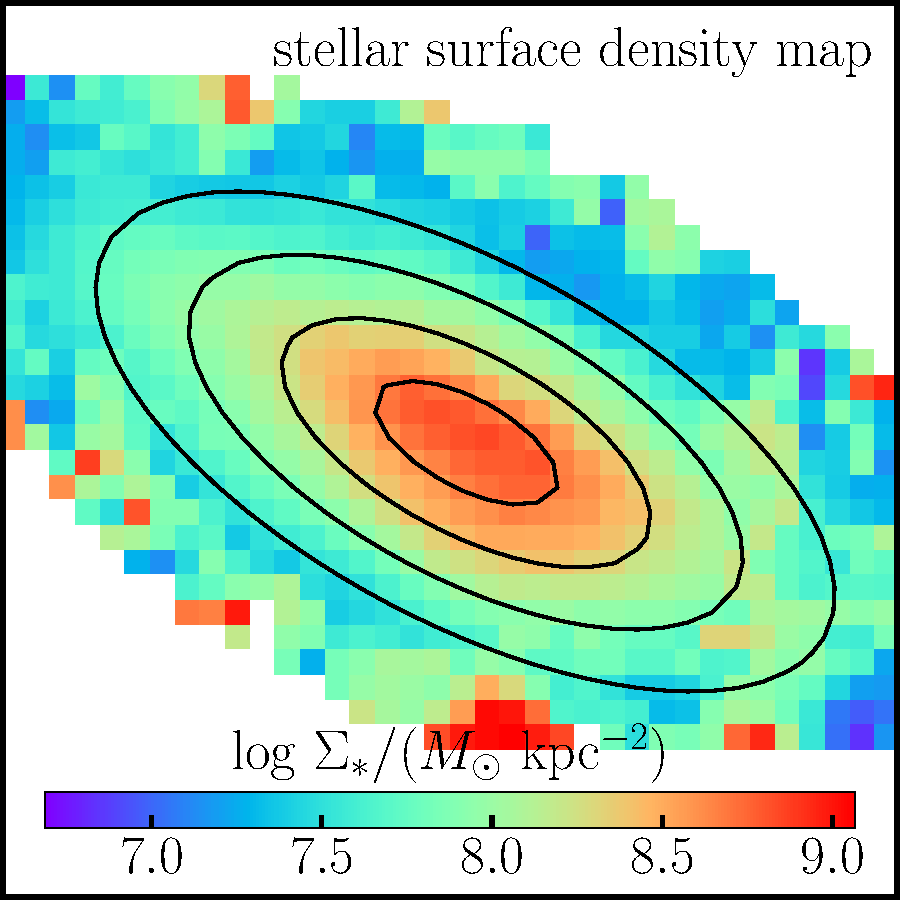
\includegraphics[width=.16\textwidth]{fig/physmap_lSDstar_ID03751.pdf}
    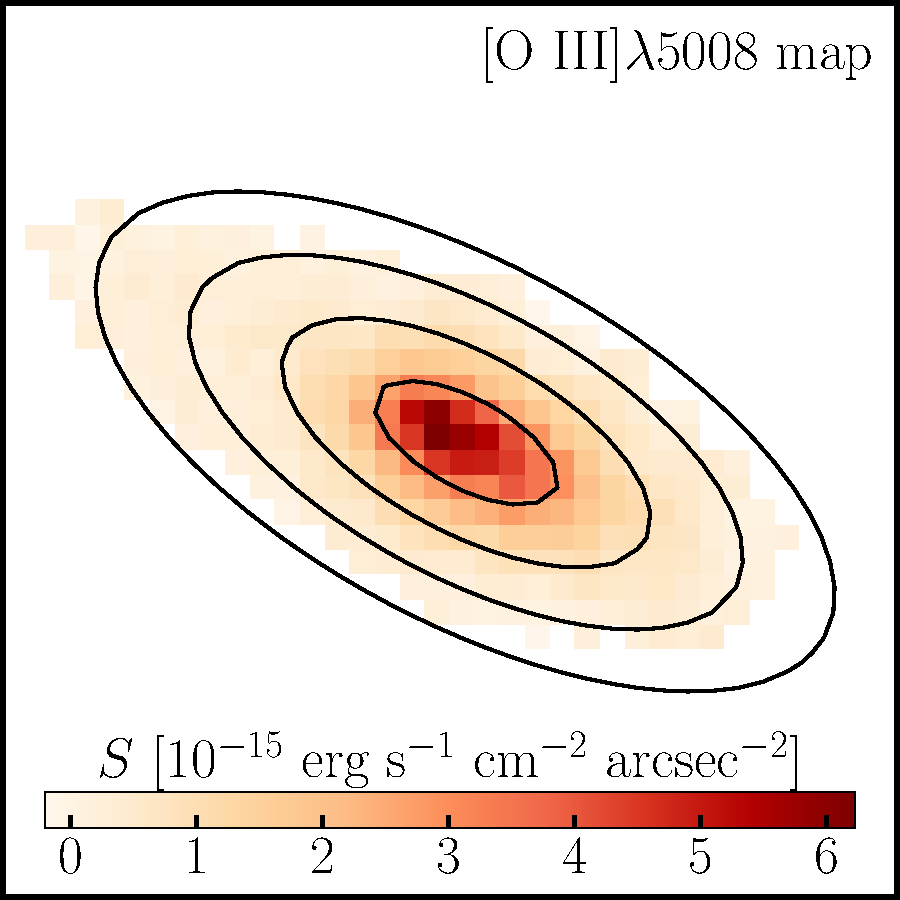
\includegraphics[width=.16\textwidth]{fig/combELmap_OIII_ID03751.pdf}
    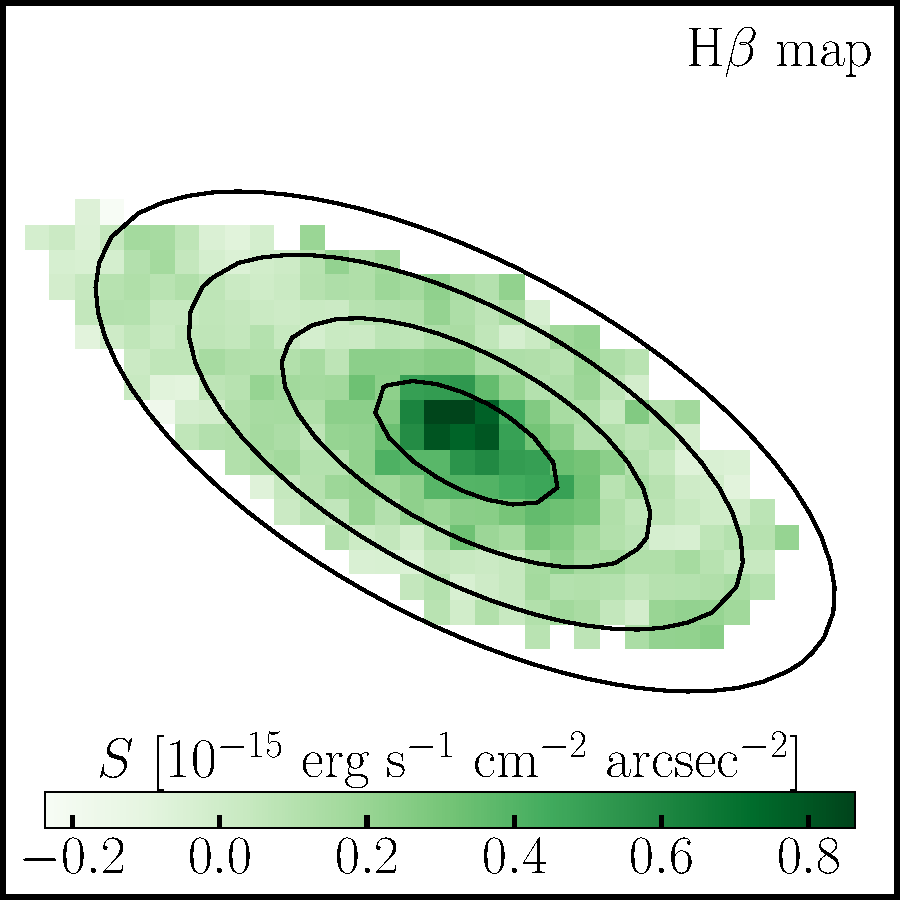
\includegraphics[width=.16\textwidth]{fig/combELmap_Hb_ID03751.pdf}
    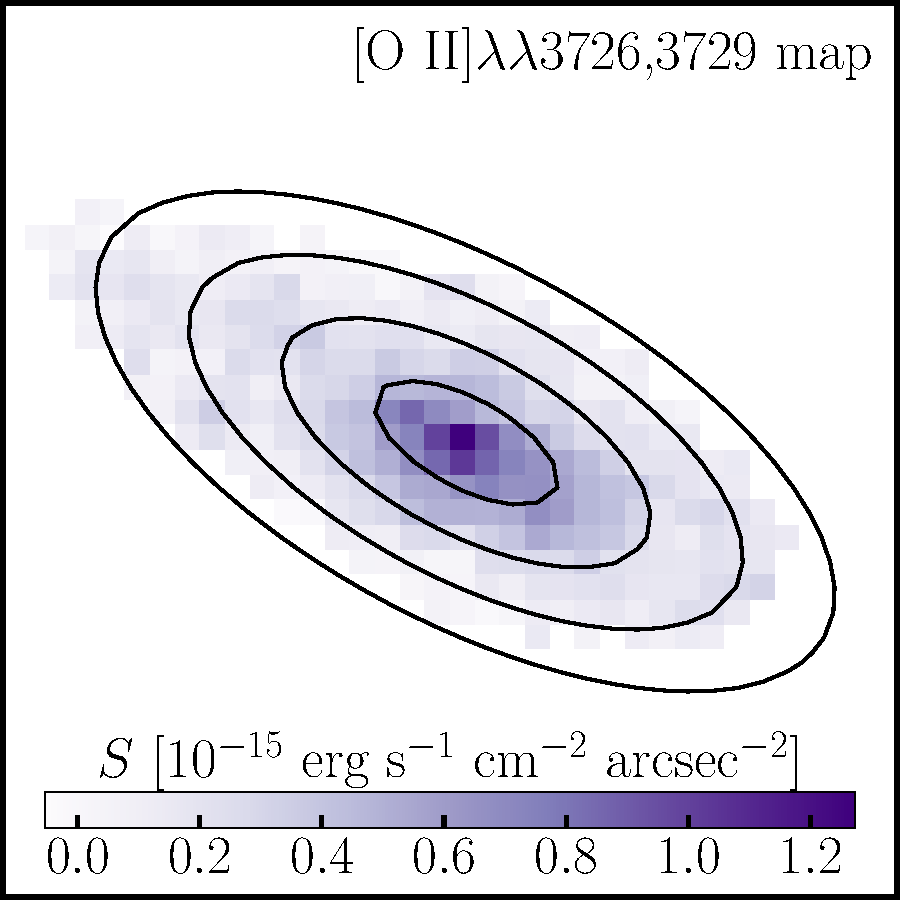
\includegraphics[width=.16\textwidth]{fig/combELmap_OII_ID03751.pdf}
    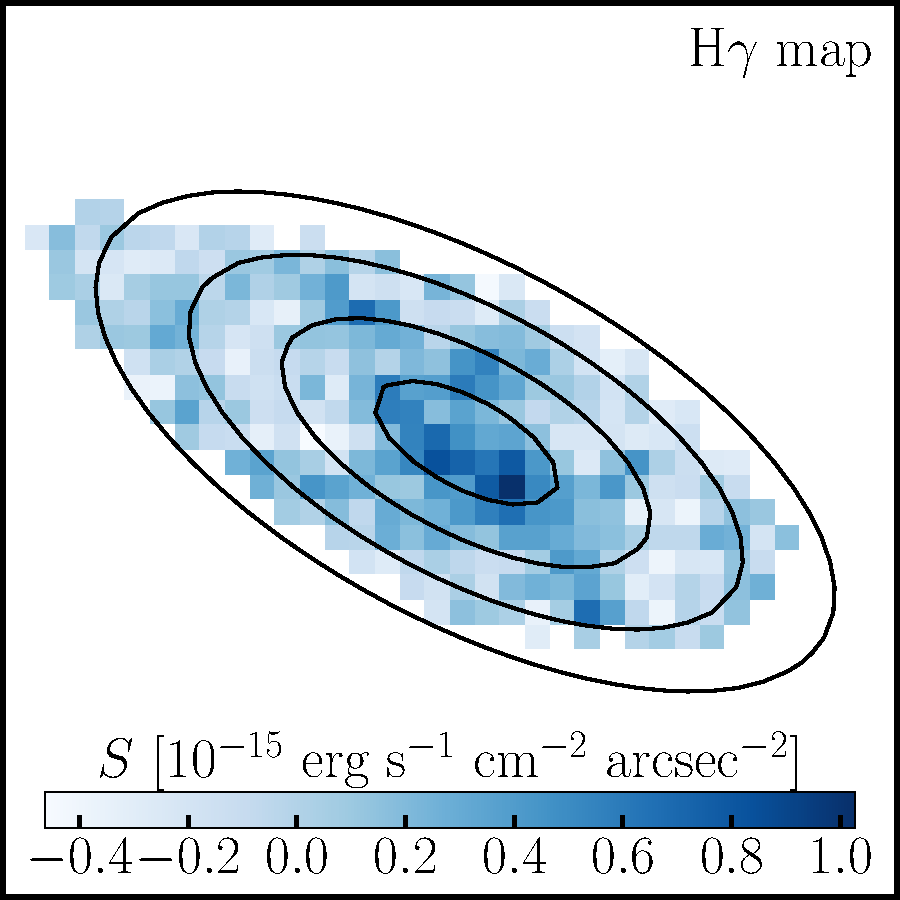
\includegraphics[width=.16\textwidth]{fig/combELmap_Hg_ID03751.pdf}\\
    \includegraphics[width=.16\textwidth]{fig/rgbstamp_ID01203.pdf}
    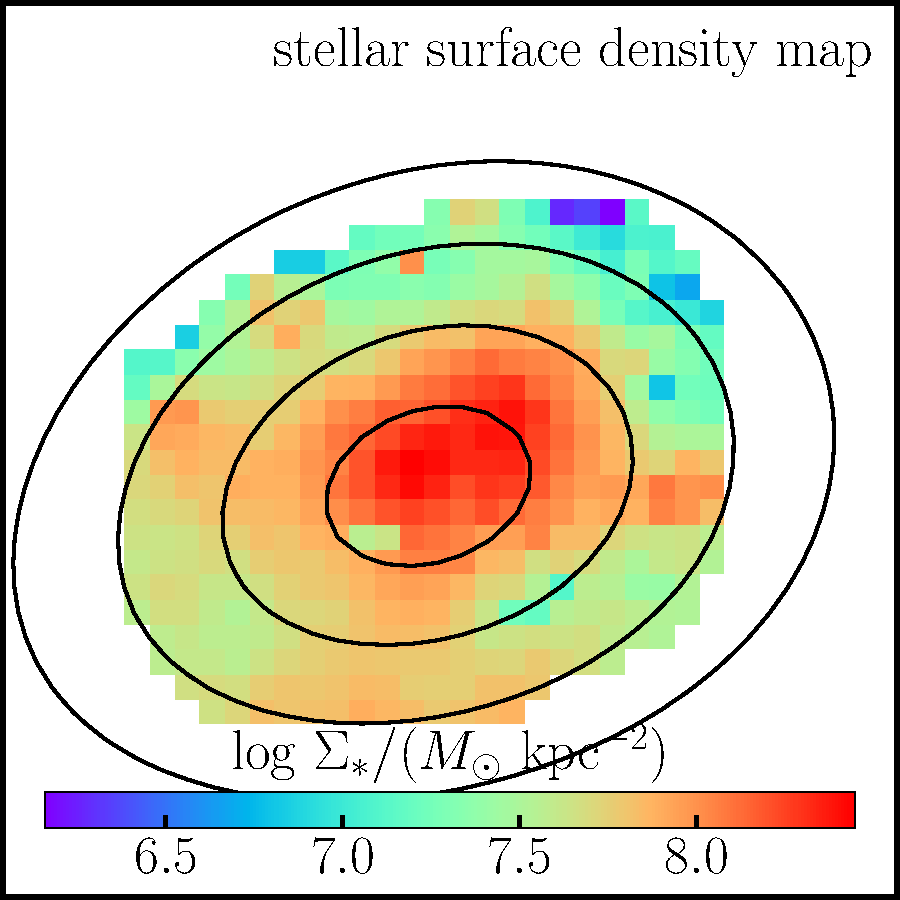
\includegraphics[width=.16\textwidth]{fig/physmap_lSDstar_ID01203.pdf}
    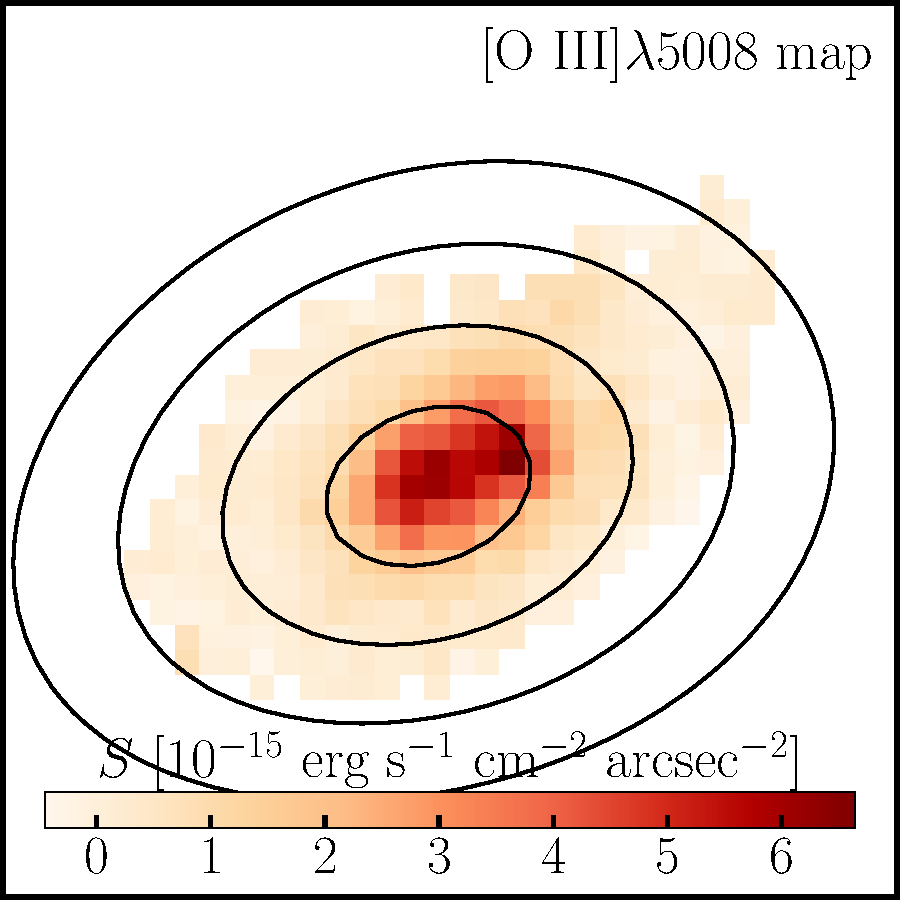
\includegraphics[width=.16\textwidth]{fig/combELmap_OIII_ID01203.pdf}
    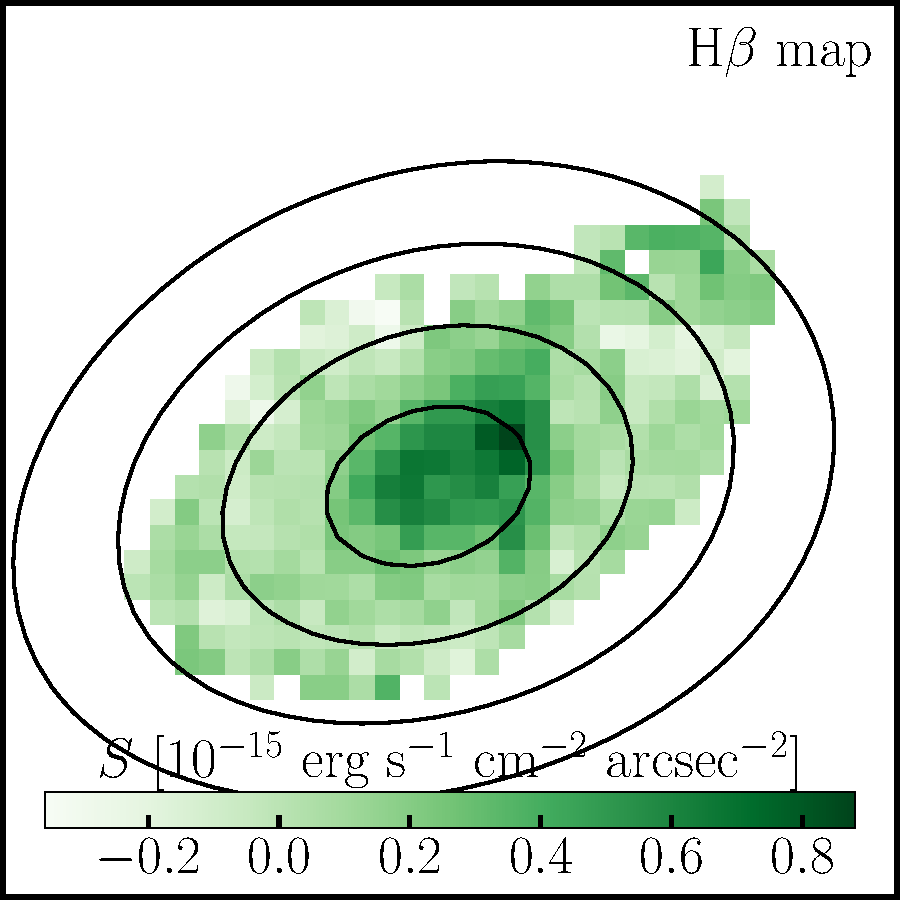
\includegraphics[width=.16\textwidth]{fig/combELmap_Hb_ID01203.pdf}
    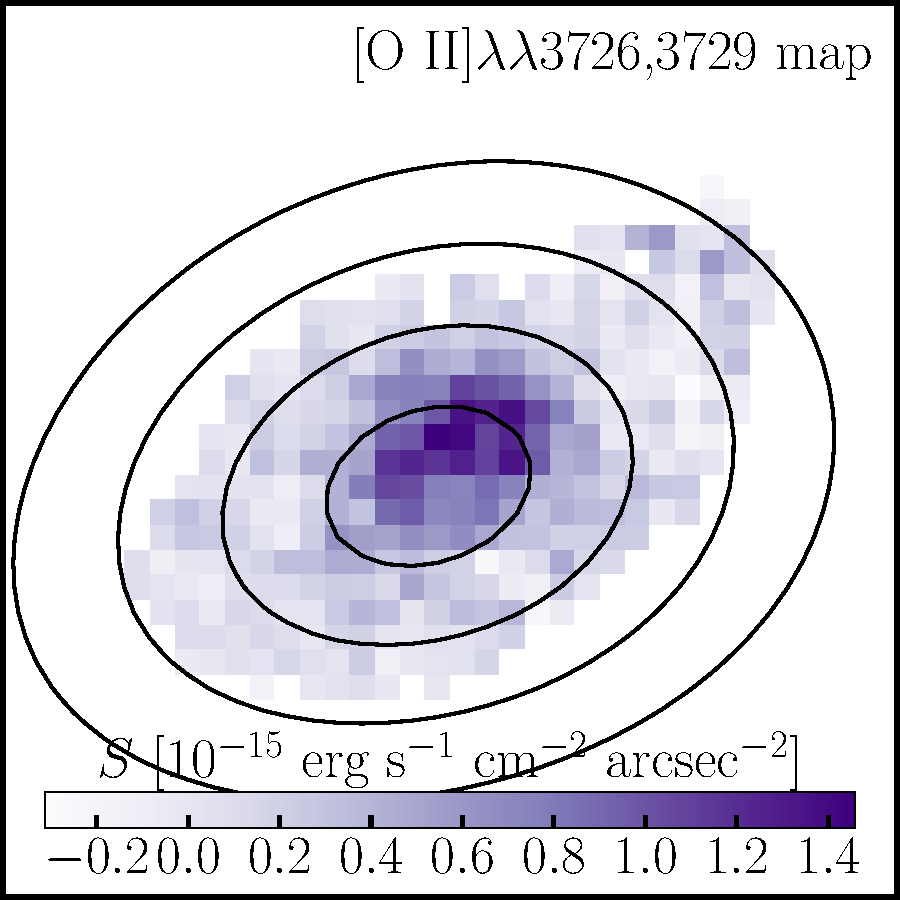
\includegraphics[width=.16\textwidth]{fig/combELmap_OII_ID01203.pdf}
    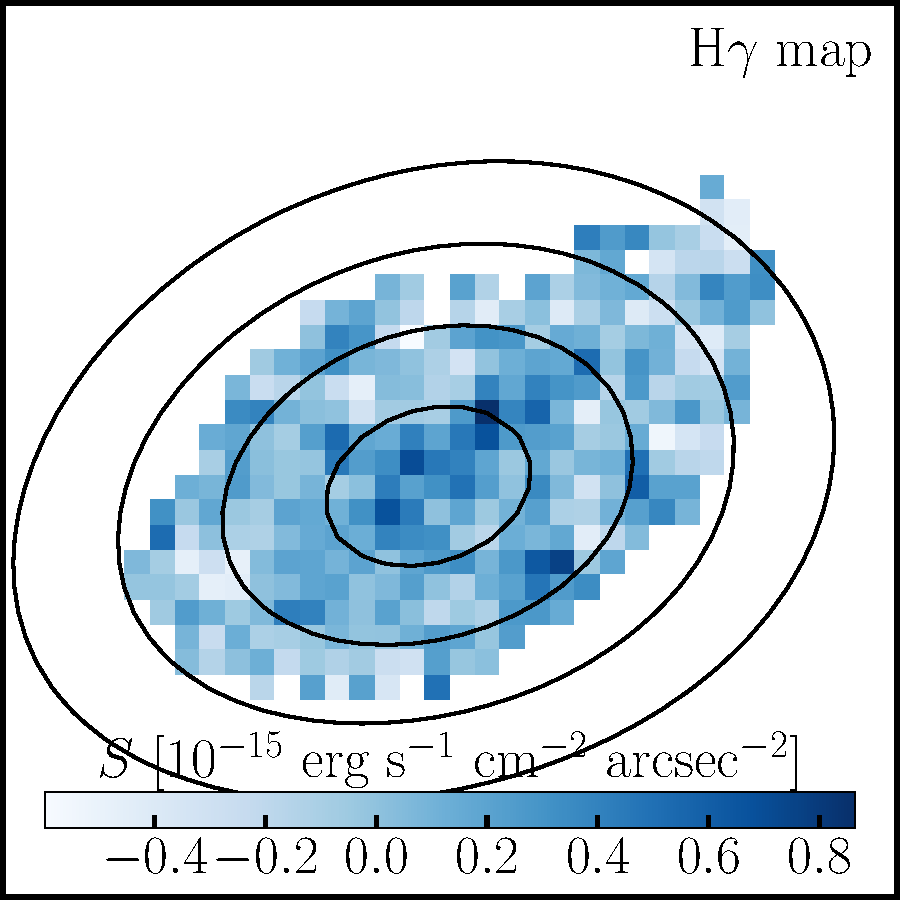
\includegraphics[width=.16\textwidth]{fig/combELmap_Hg_ID01203.pdf}
    \caption[Two star-forming dwarf galaxies at $z$$\sim$2 displaying unusually strong inverted metallicity gradients]{Two star-forming dwarf galaxies at $z$$\sim$2 displaying unusually strong inverted metallicity gradients, securely
    determined at sub-kpc spatial resolution. For each source we show, from left to right: color composite image (created from
    \hst broad-band photometry), stellar surface density map (obtained from SED fitting to \hst photometry), and surface
    brightness map of ELs \OIII, \Hb, \OII, and \Hg. The black contours overlaid represent the source plane de-projected
    galacto-centric radii with 1 kpc interval. The two light-dispersion directions for the grism exposures are 
    denoted by the orange and cyan arrows (see Figures~\ref{fig:3751spec} and \ref{fig:1203spec} for the 
    corresponding spectra).
    The spatial extent and orientation are unchanged for the two sources in all 2D
    stamps throughout. North is up and east is to the left.
    \label{fig:combELmap}}
\end{figure}
%= = = = = = = = = = = = = = = = = = = = = = = = = = = = = = = = = = = = = = = =

\section{Methods and Results}\label{sect:rslt}

In this section, we describe our key methods used to derive radial metallicity gradients (Section~\ref{sect:metalgrad}), 2D maps 
of \SFR, average stellar population age, and gas fraction (Section~\ref{sect:physprop}), as well as spatial 
distributions of net gaseous outflow rate and mass loading factor (Section~\ref{sect:regulator}).
The main results are presented alongside the corresponding methods.


\subsection{Radial Metallicity Gradients}\label{sect:metalgrad}

Since we infer metallicity from strong line flux ratio diagnostics, calibrated by either empirical methods, or 
theoretical methods, or a hybrid of both, it is essential to make sure that the line emission is not 
contaminated by active galactic nucleus (AGN) ionization or shock excitation.
As shown in Figure~\ref{fig:bluediagram}, we verify that our targets have a low probability (<\%10) of being 
classified as AGNs according to the mass-excitation diagram \citep{Juneau:2014ca}.
Their individual radial annuli also have excitation and ionization states, as revealed in their loci in the 
$f_{\OIII}/f_{\Hb}$ versus $f_{\OII}/f_{\Hb}$ diagram and the O$_{32}$(=$f_{\OIII}/f_{\OII}$) versus 
R$_{23}$(=$(f_{\OIII~5008} + f_{\OIII~4960} + f_{\OII})/f_{\Hb}$) diagram,
compatible with \HII regions \citep{Lamareille:2004jk,Rodrigues:2012dr,2015ApJ...813..126J}.
In the source ID01203 covered by our follow-up \osiris observations (see Appendix~\ref{sect:kinem}), its 
integrated $f_{\NII}/f_{\Ha}$ ($\lesssim0.1$ at 3-$\sigma$) also shows no sign of AGN or shocked gas emission.

%= = = = = = = = = = = = = = = = = = = = = = = = = = = = = = = = = = = = = = = =
%%% Figures
\begin{figure}
    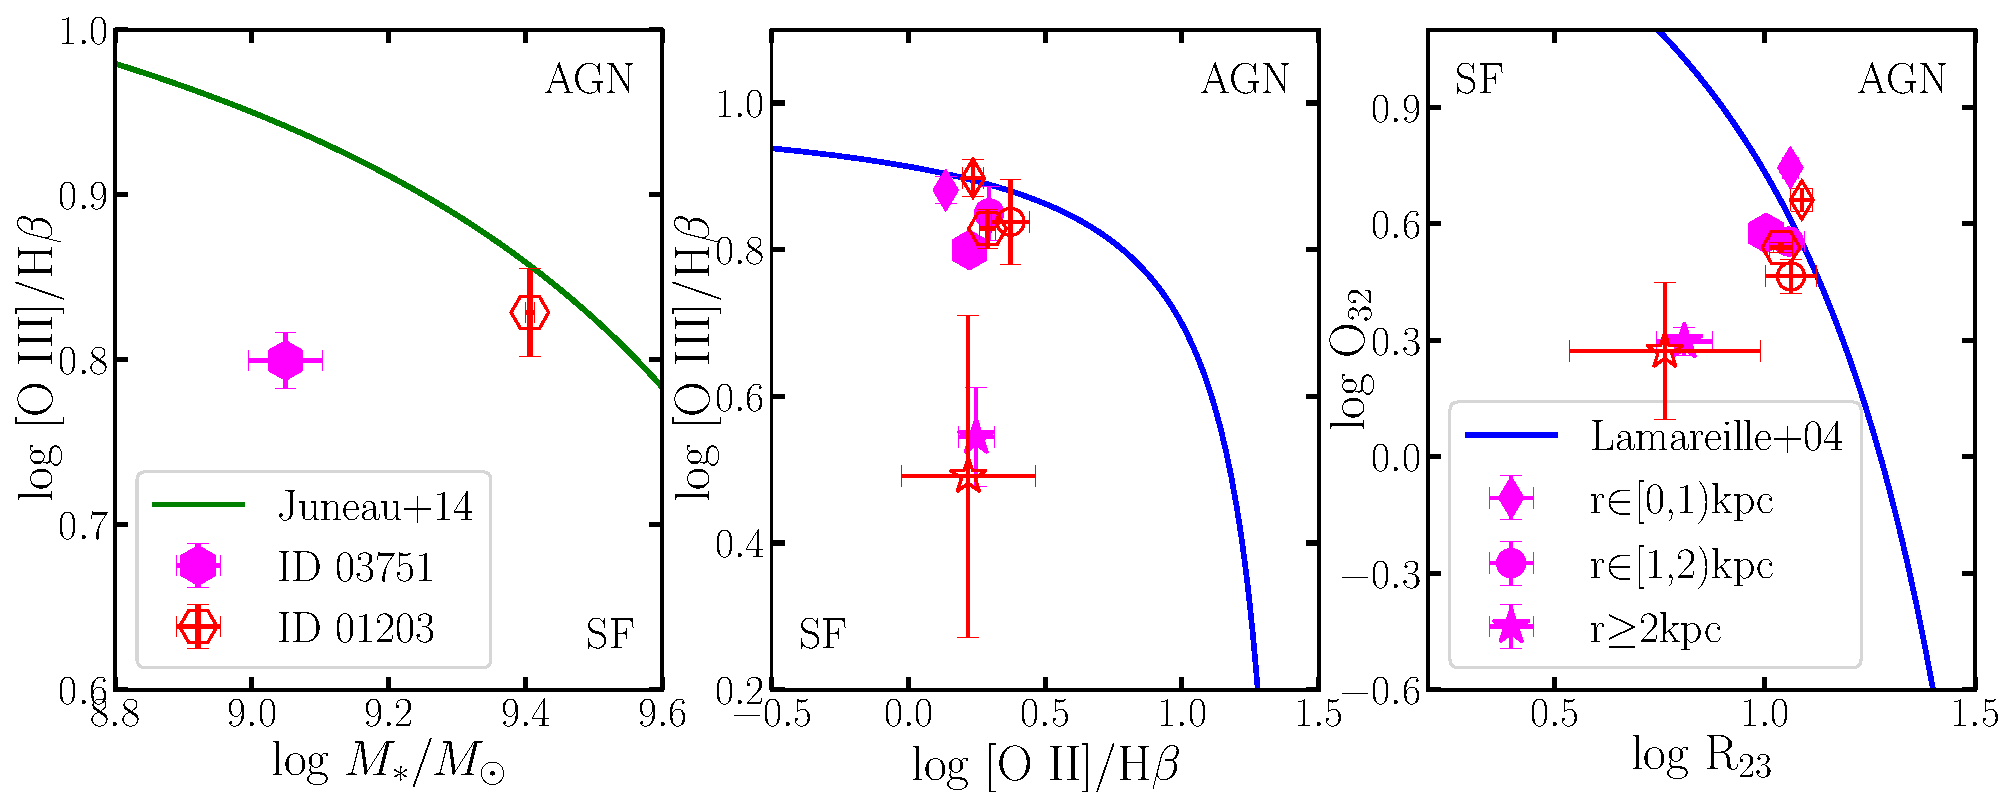
\includegraphics[width=\textwidth]{fig/bluediagram.pdf}
    \caption[The diagnostic diagrams for our sources.]{The diagnostic diagrams for our sources.
    On the left, we show the mass-excitation diagram
    with the demarcation scheme between the loci of AGNs and 
    star-forming (SF) galaxies proposed in \citet{Juneau:2014ca}. Our galaxies can be safely classified as the 
    latter.
    In the middle and right panels, we show the ``blue'' diagrams with the boundaries described by \citet{Lamareille:2004jk}.
    Following the conventions in the left panel, we use filled symbols to represent measurements for ID03751 
    whilst empty ones for ID01203.
    Furthermore, the hexagons correspond to the measurements integrated over the entire galaxies (as in the left 
    panel), whereas the other symbols denote results obtained in different radial annuli, as explained in the 
    legend of the right panel.
    Again we see that the contamination from AGN ionization is minimum for our sources, even in the central 
    regions.
    The two galaxies presented in this work share similar evolutionary trends in their excitation and ionization 
    states with respect to galacto-centric radius, in addition to the strongly inverted radial gradient in 
    metallicity (see Figure~\ref{fig:oh12grad}).
    \label{fig:bluediagram}}
\end{figure}
%= = = = = = = = = = = = = = = = = = = = = = = = = = = = = = = = = = = = = = = =

Our measurements of radial \mgs largely follow the procedures described in our previous work \citep{Wang:2016um}.
We use a Bayesian approach to jointly infer metallicity (\oh), nebular dust extinction ($\Av^{\rm N}$), and de-reddened \Hb flux
($f_{\Hb}$).  We explore the parameter space using the Markov Chain Monte Carlo sampler \emc\citep{ForemanMackey:2013io}.
The likelihood function is given by $\mathrm{L}\propto\exp(-\chisq/2)$ with
\begin{align}
    \chisq = \sum_i \frac{\(f_{\el{i}} - R_i \cdot f_{\Hb}\)^2}
        {\(\sigma_{\el{i}}\)^2 + \(f_{\Hb}\)^2\cdot\(\sigma_{R_i}\)^2},
\end{align}
where \el{i} corresponds to each available EL: \OIII, \Hb, \OII, and \Hg. $f_{\el{i}}$ and $\sigma_{\el{i}}$ are the flux and uncertainty of \el{i}. $R_i$ is the flux ratio between \el{i} and \Hb, with $\sigma_{R_i}$ being the intrinsic scatter at fixed physical properties.
In the case $\el{i}=\Hg$, $R_i$ is given by the Balmer decrement $f_{\Hg}/f_{\Hb}=0.47$.
For $\el{i} \in \{\OII,~\OIII\}$, $R_i$ and $\sigma_{R_i}$ are given by the strong line metallicity diagnostics 
($f_{\OIII}/f_{\Hb}$ and $f_{\OII}/f_{\Hb}$) calibrated by \citet{2008A&A...488..463M}.
The \citet{2008A&A...488..463M} calibrations combine the direct electron temperature measurements from the Sloan 
Digital Sky Survey in the low-metallicity (\oh<8.35) branch \citep{2006A&A...459...85N} and the photoionization 
model predictions in the high-metallicity (\oh>8.35) branch \citep{Kewley:2002ep}, providing a continuous and 
coherent recipe over a wide metallicity range.
We also adopt the empirical calibrations by \citet{Curti:2016fn} based on metallicities given by pure electron
temperature method, and verified that there is no significant change in our gradient measurements.
The same process is applied to both galaxy-integrated fluxes and to fluxes measured at individual spatial pixels 
(spaxels).


To obtain the correct intrinsic de-projected distance scale for each spaxel, we conducted full source plane morphological
reconstruction of our sources.
%Since our targets are gravitationally lensed, we must account for lensing magnification to determine their true morphologies and
%global properties. We note that surface densities and flux ratios (used to determine metallicity) are unaffected by
%lensing.
We ray-trace the image of each galaxy to its source plane using up-to-date lens models for each cluster: the macroscopic
model of \SJ version 4 for \clsan \citep{Johnson:2014cf}, and the \textsc{Zitrin} version 2 model for \clba
\citep{2015ApJ...801...44Z}. Other lens models are available for these clusters 
\cite[\eg][]{Diego:2016ww,Strait:2018ul} and we verified that the morphology of each source
is robust to the choice of model.

For each source, we fit the SED of individual spaxels using the procedures described in Section~\ref{sect:data}, 
obtaining the 2D stellar surface density (\Sstar) map shown in Figure~\ref{fig:combELmap}. Then we reconstruct 
\Sstar map in the source plane by de-lensing the surface densities according to the deflection field given by the 
macroscopic lens models.
To minimize the stochasticity in stellar population synthesis \citep{Fouesneau:2010ea,Eldridge:2012ds}, 
we make sure that the source plane resolution elements during this reconstruction contain enough stellar masses 
($\gtrsim 10^5$ \Msun) to be representative of complete stellar populations.
The axis ratios, inclinations, and major axis orientations are determined from an elliptical Gaussian fit. This 
procedure provides the intrinsic lensing-corrected morphology, and in particular, the galacto-centric radius at 
each point of the observed images.
The radial scale as black contours in all figures is used to establish the absolute metallicity gradient slope (i.e., in units of 
dex per proper kpc).
From the source reconstructed morphology, we measure their effective radius where the enclosed mass 
reaches half the total mass of the source. The measurements are represented by $R_{\rm eff}$ in 
Table~\ref{tab:srcprop}.

Figure~\ref{fig:oh12grad} shows the 2D maps of metallicity of our selected two dwarf galaxies at $z\sim2$.
Clearly, the outskirts of our galaxies display highly elevated oxygen abundance ratios.
In particular, the outskirts of ID03751 are more metal enriched by $\sim$0.4 dex (\ie a factor of 2.5) than its center, and more 
metal-rich by $\sim$0.2 dex than the value inferred based on the fundamental metallicity relation (FMR) given its 
integrated \Mstar \cite{2010MNRAS.408.2115M,Mannucci:2011be}.
Note that our metallicity measurements extend beyond the source effective radius to cover large enough 
dynamic range, but not into the region where a plateau/flattening in metallicity \citep[\ie, at $R>2-2.5 R_{\rm 
eff}$,][]{2014A&A...563A..49S,SanchezMenguiano:2016gj,Molla:2018em} is likely to occur, which might bias the 
overall gradient determination.
For the first time, we are able to detect strongly inverted metallicity gradients in $z$$\sim$2 dwarf galaxies
at unprecedentedly high confidence: 0.122$\pm$0.008 dex/kpc for ID03751 ($\sim15.2\sigma$), and
0.111$\pm$0.017 dex/kpc for ID01203 ($\sim6.5\sigma$).

The question is thus what caused these dwarf galaxies to have such strongly inverted gradients?
First of all, our sources show no evidence of major mergers, supported by their regular morphology displayed in the 2D maps of 
\Mstar and EL surface brightness in Figure~\ref{fig:combELmap}.
For source ID01203 with \osiris data, this statement is further strengthened by the kinematic evidence of disk orderly rotation.
Secondly, the fact that the outskirts of our sources show elevated metallicity as compared to the FMR 
expectations indicates that there are more metals in the outer regions than could be produced by the stars in those 
regions.
This discourages any explanations involving solely low-metallicity gas inflows, not limited to those induced by mergers.
In the subsequent sections, we thus gather all available pieces of observational evidence to further investigate the possible 
cause.

%= = = = = = = = = = = = = = = = = = = = = = = = = = = = = = = = = = = = = = = =
%%% Figures
\begin{figure}
    \centering
    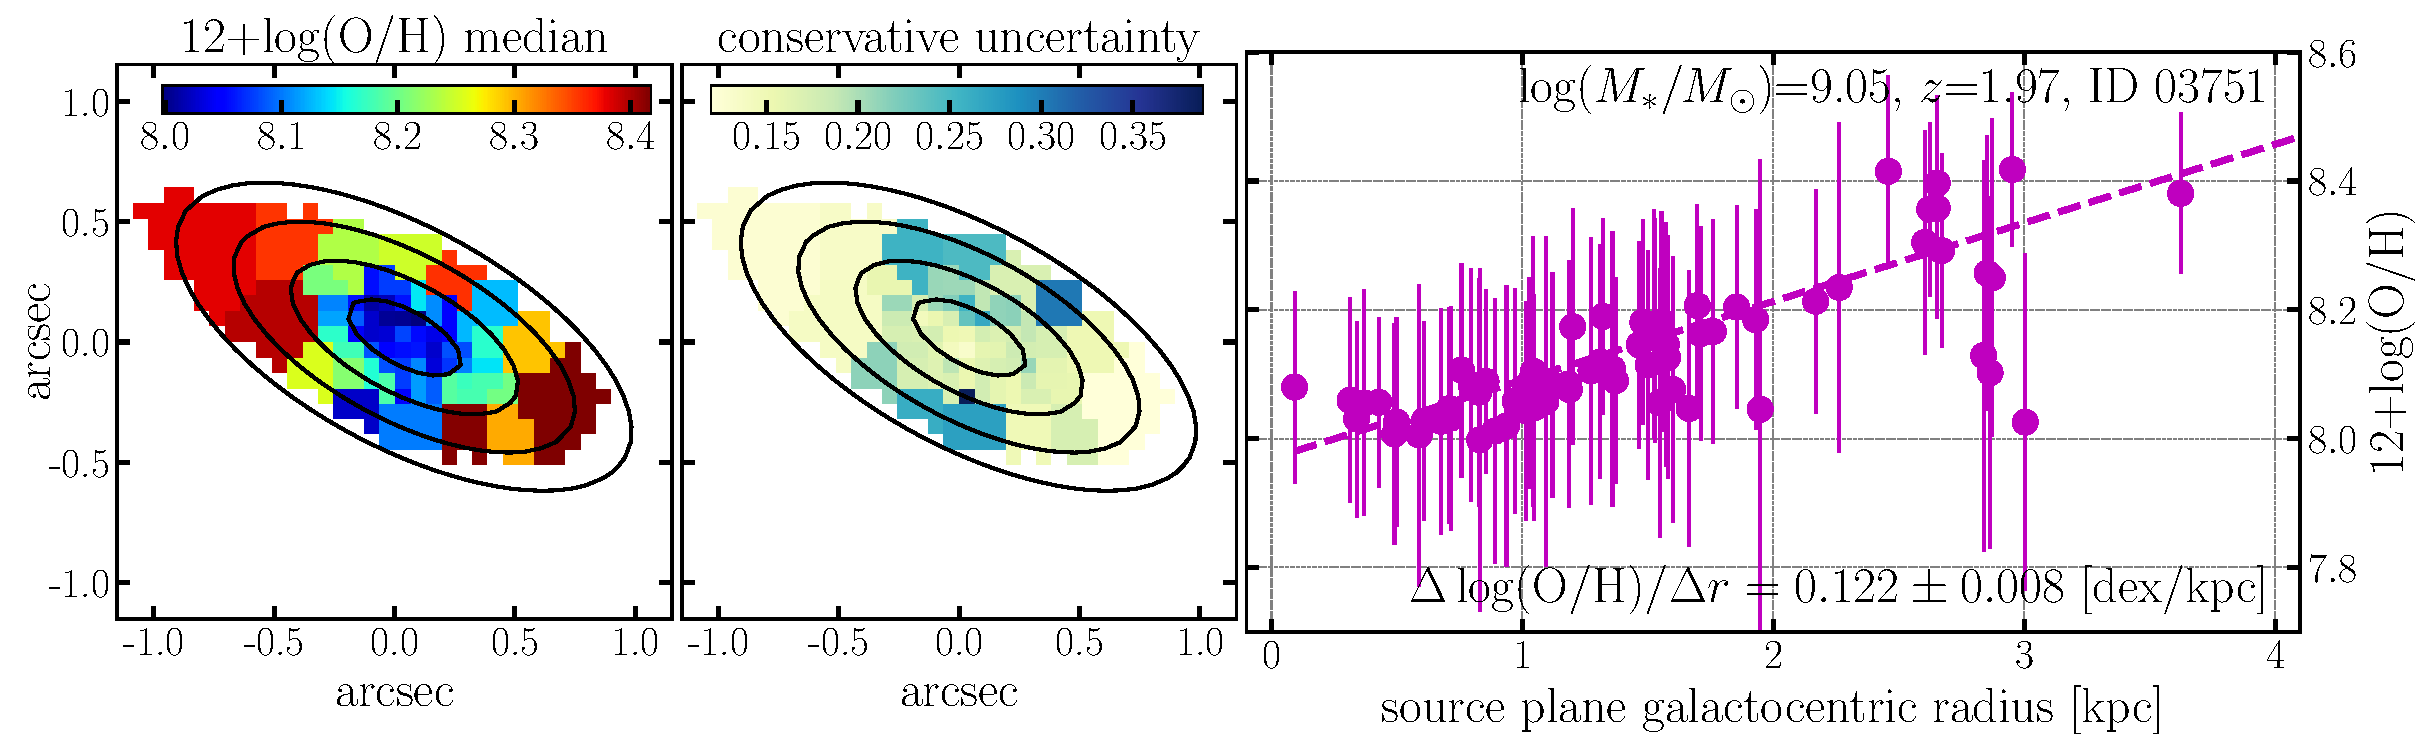
\includegraphics[width=\textwidth]{fig/metalgrad_ID03751.pdf}\\
    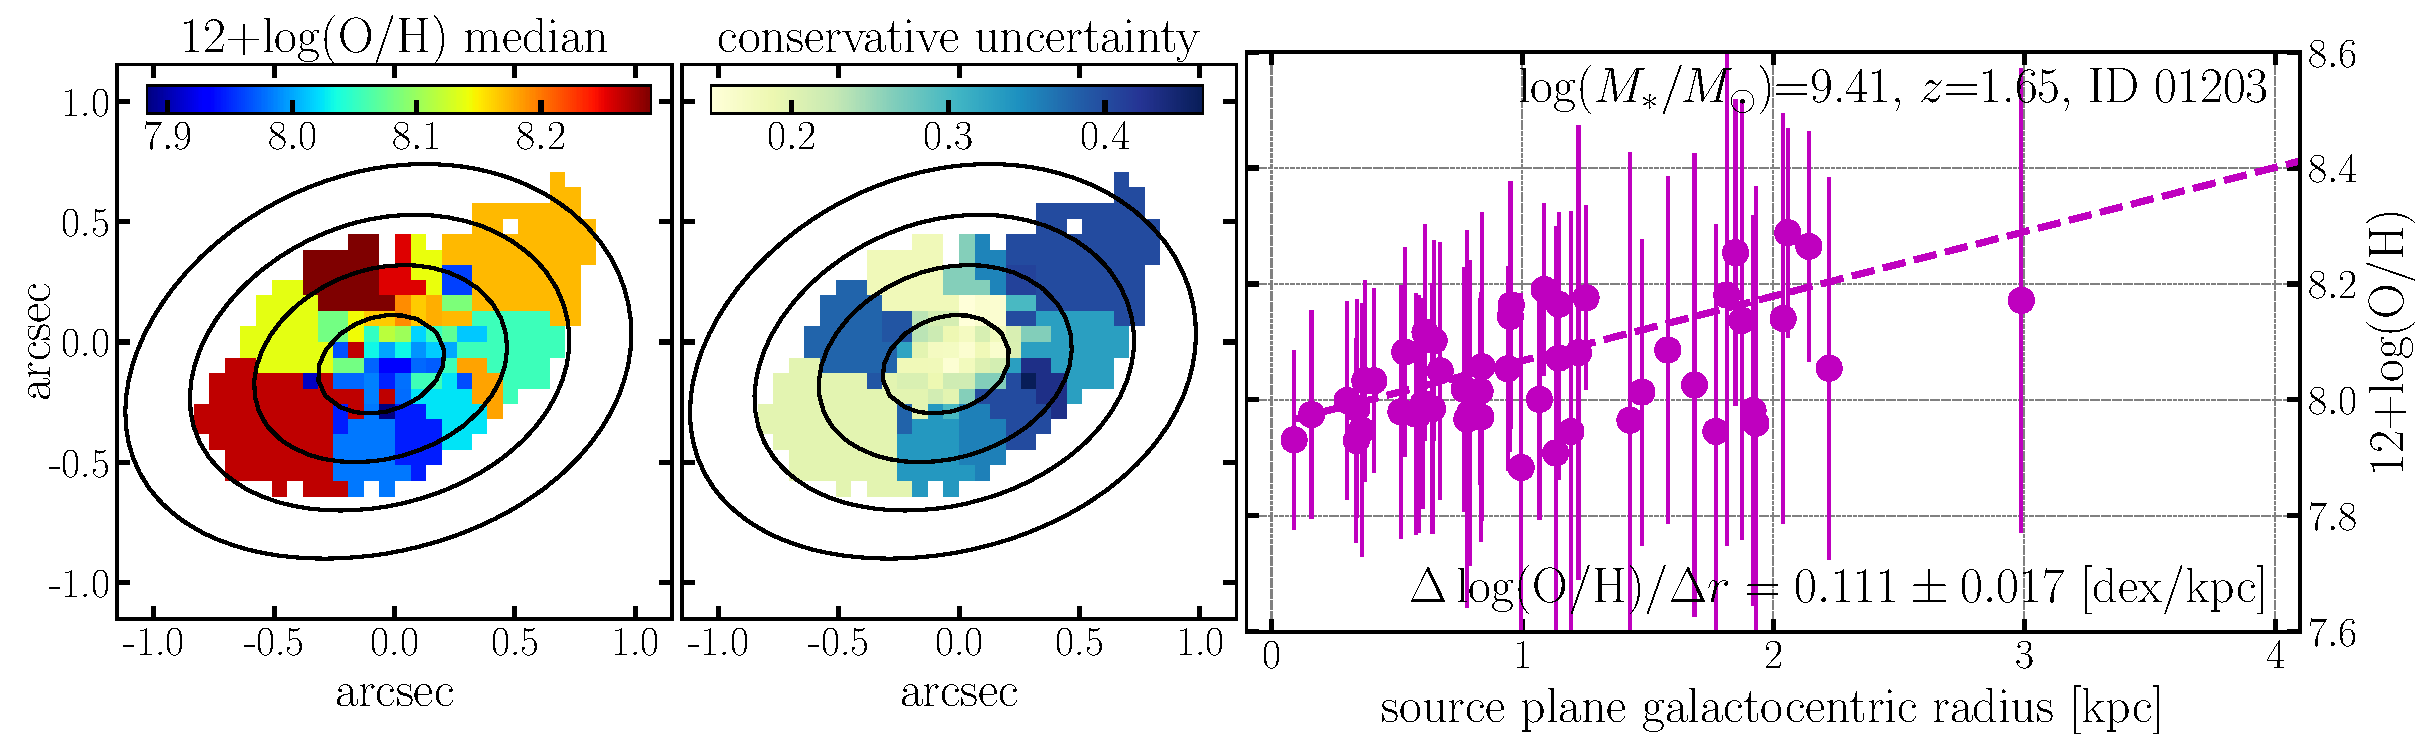
\includegraphics[width=\textwidth]{fig/metalgrad_ID01203.pdf}
    \caption[Metallicity maps and radial gradient measurements of the two galaxies.]
    {Metallicity maps and radial gradient measurements of the two galaxies. The left panels show the 2D maps of the median
    value estimates of metallicity, and the central panels show their conservative uncertainties (\ie the larger side of the
    asymmetric 1-$\sigma$ error bars). The right panels show the corresponding radial gradients measurements.
    The black contours again mark the source plane de-projected galacto-centric distances as in 
    Figure~\ref{fig:combELmap}.
    We adopted weighted Voronoi tessellation \citep{Cappellari:2003eu,Diehl:2006cz},
    with a SNR of 10 on \OIII for the binned metallicity maps.
    In the right column, these bins are plotted as individual data points.
    The dashed line denotes the linear regression from these points, with the measured radial slope shown at the bottom of each
    panel.  For both galaxies, the radial gradient is strongly positive (\ie inverted).
    \label{fig:oh12grad}}
\end{figure}
%= = = = = = = = = = = = = = = = = = = = = = = = = = = = = = = = = = = = = = = =


\subsection{\SFR, Stellar Population Age, and Gas Fraction}\label{sect:physprop}

To understand the cause of the strongly inverted metallicity gradients seen in these dwarf galaxies,
we combine their EL maps with \hst broad-band photometry to derive 2D maps of \Mstar, \SFR,
stellar population age, and gas surface density for each galaxy.
The \SFR is derived from extinction-corrected Balmer emission line flux. Maps of \Hb and \Hg emission are shown in
Figure~\ref{fig:combELmap}. The \Hb/\Hg line ratio provides a measurement of nebular extinction although it is limited by the
modest signal-to-noise of \Hg. We obtain more precise results from \hst photometry, by converting \B-\I color maps to spatial
distributions of stellar reddening $E_{\rm S}(B-V)$ \citep{Daddi:2004hj}. Nebular reddening $E_{\rm N}(B-V)$ is then calculated
following \citet{Valentino:2017by}.  The nebular reddening maps of both our galaxies show lower dust attenuation in centers than
that in outskirts, consistent with the inverted metallicity gradients shown in Figure~\ref{fig:oh12grad}.

We calculate extinction in \Hb adopting a \citet{1989ApJ...345..245C} dust extinction law
(with \Rv=3.1) and assuming Case B recombination with Balmer ratios appropriate for fiducial \HII region properties (\ie,
\Ha/\Hb~=~2.86).  Finally, we convert intrinsic \Ha luminosity to \SFR through the commonly used calibration
\citep{Kennicutt:1998ki},
\begin{align}
    {\rm SFR} = 4.6\times10^{-42}~ \frac{L(\Ha)}{\rm erg/s} \quad [\Msun/\textrm{yr}],
\end{align}
appropriate for the \citet{Chabrier:2003ki} IMF.
This provides the instantaneous star formation rate on $\sim$10 Myr time scales; we note that the ultraviolet continuum probed by
\hst photometry is sensitive to recent \SFR over a longer time span ($\sim$100-300 \Myr). The short timescales probed by Balmer
emission are most relevant for determining outflow physical properties, which are highly dynamic on small spatial scales, \eg, at 
sub-kpc level.
%($v_{\rm wind}\gtrsim v_{\rm circ}$, $<1$ \kpc scales).

Next we derive average stellar age maps, using the spatial distribution of EL EW as the primary constraint. We
calculate \Hb rest-frame EWs from our maps of the emission line flux and stellar continuum flux density. Stellar continuum maps
are corrected for emission line contamination as described in Section~\ref{sect:data}. We correct for stellar Balmer absorption
which we estimate to be rest-frame EW~$\sim$3 \AA\ in \Hb based on the derived galaxy properties \citep{Kashino:2013ev}.  Maps of
\Hb EW are then converted to average stellar age using a series of \burst stellar population synthesis
models \citep{Leitherer:1999jt,Zanella:2015ej} assuming 1/5 solar metallicity and constant star formation history.

We also compare the age estimates given by our SED fitting (Section~\ref{sect:data}) and \Hb rest-frame EW using the method
described above. The median values given by the former practice are systematically larger than those of the latter by $\sim$0.5
dex, but we note that the uncertainties by the SED fitting are usually much larger due to the absence of prominent continuum
spectral age indicators, \eg, \Dn and \HdA \citep{Kauffmann:2003cu}. Hence, we adopt the results from \Hb rest-frame EW as the
average age for stellar populations throughout our paper, as we consider this a more reliable estimate.

Finally, we calculate the gas fraction defined as
\begin{align}
    \fgas=\Sgas/\left(\Sgas+\Sstar\right).
    \label{eq:fgas}
\end{align}
Since we do not directly observe the bulk of interstellar gas, we instead estimate gas surface density \Sgas by 
inverting the
Kennicutt-Schmidt (KS) law \citep{Schmidt:1959bp,Kennicutt:1998id}, \ie, $\Sigma_{\SFR}\propto\Sgas^{N}$ together with our
measurements of $\Sigma_{\SFR}$ described above.  We adopt the more robust extended version of the KS law developed by 
\citet{Shi:2011ck,Shi:2018wf} which is especially useful in low density regimes:
\begin{align}
    \frac{\Sigma_{\SFR}}{\Msun/\yr/\kpc^2} = 10^{-4.76} \left(\frac{\Sstar}{\Msun/\pc^2}\right)^{0.545}
    \left(\frac{\Sgas}{\Msun/\pc^2}\right)^{1.09}.
    \label{eq:KSlaw}
\end{align}
This extended KS law has been tested in numerous ensembles of galaxies as well as low surface brightness regions in individual
galaxies, and is shown to have relatively small scatter ($\sim$0.3 dex) over a large dynamic range of gas and \SFR surface
densities. We have combined in quadrature this systematic uncertainty of 0.3 dex in our estimates of \Sgas.

Figure~\ref{fig:physmap} shows the derived 2D maps of \SFR, average stellar age, and gas fraction.
In general, we observe centrally concentrated star formation, with the most actively star-forming regions having surface densities 
$\gtrsim10~\Msun/\yr/\kpc$.
On average, the central regions also have older stellar populations and smaller gas fractions than the outskirts, indicating that
the outer regions are still in the early stages of converting their gas into stars.
These features together indicate that we are witnessing the rapid build-up of galactic disks through in-situ star formation and 
strongly support an inside-out mode of galaxy growth \citep{Nelson:2014is,2013ApJ...765...48J}.

%= = = = = = = = = = = = = = = = = = = = = = = = = = = = = = = = = = = = = = = =
%%% Figure:
\begin{figure}
    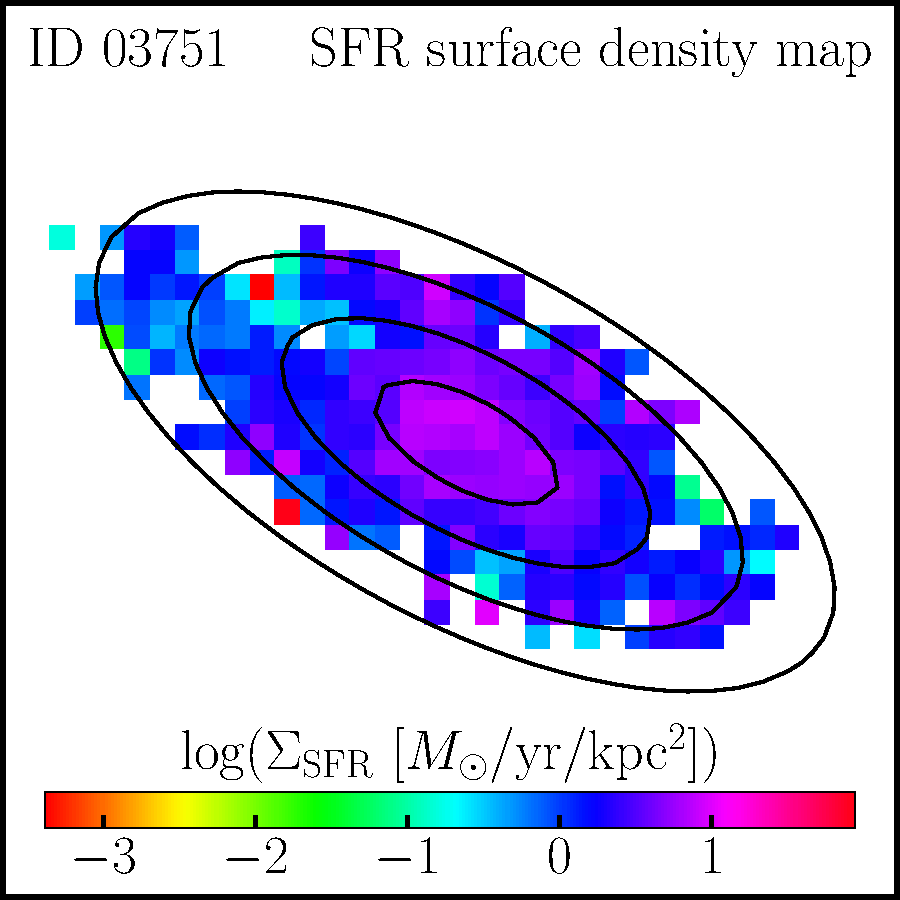
\includegraphics[width=.33\textwidth]{fig/physmap_lsfr_ID03751.pdf}
    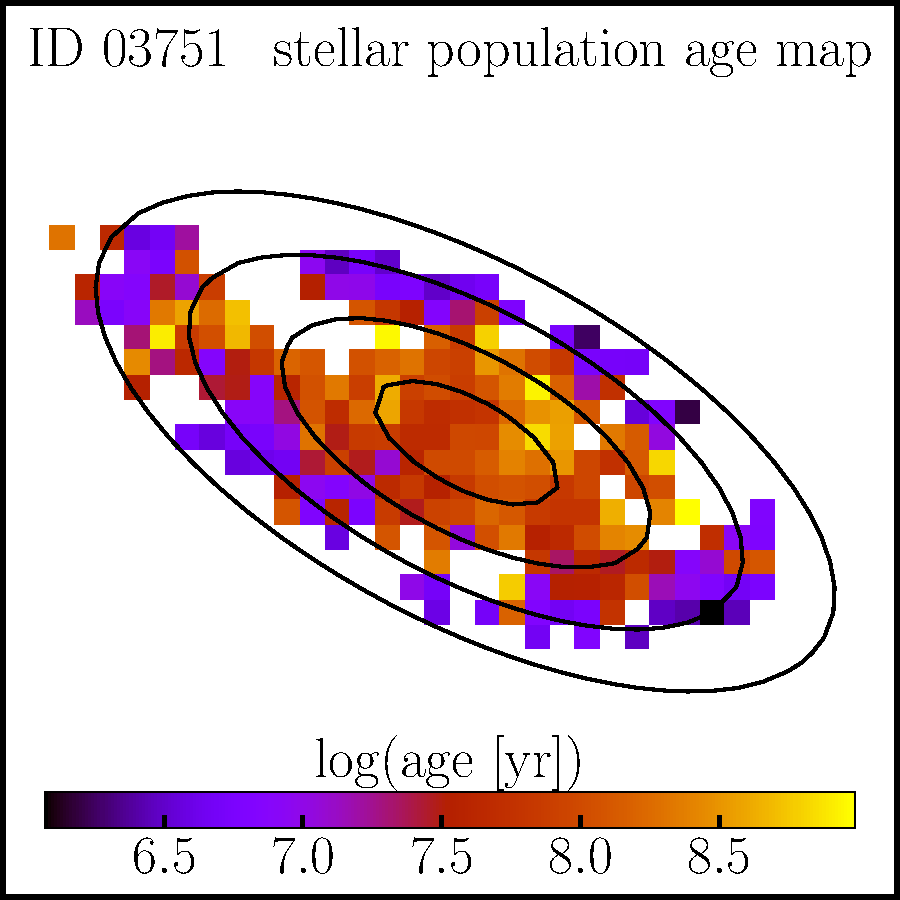
\includegraphics[width=.33\textwidth]{fig/physmap_lage_ID03751.pdf}
    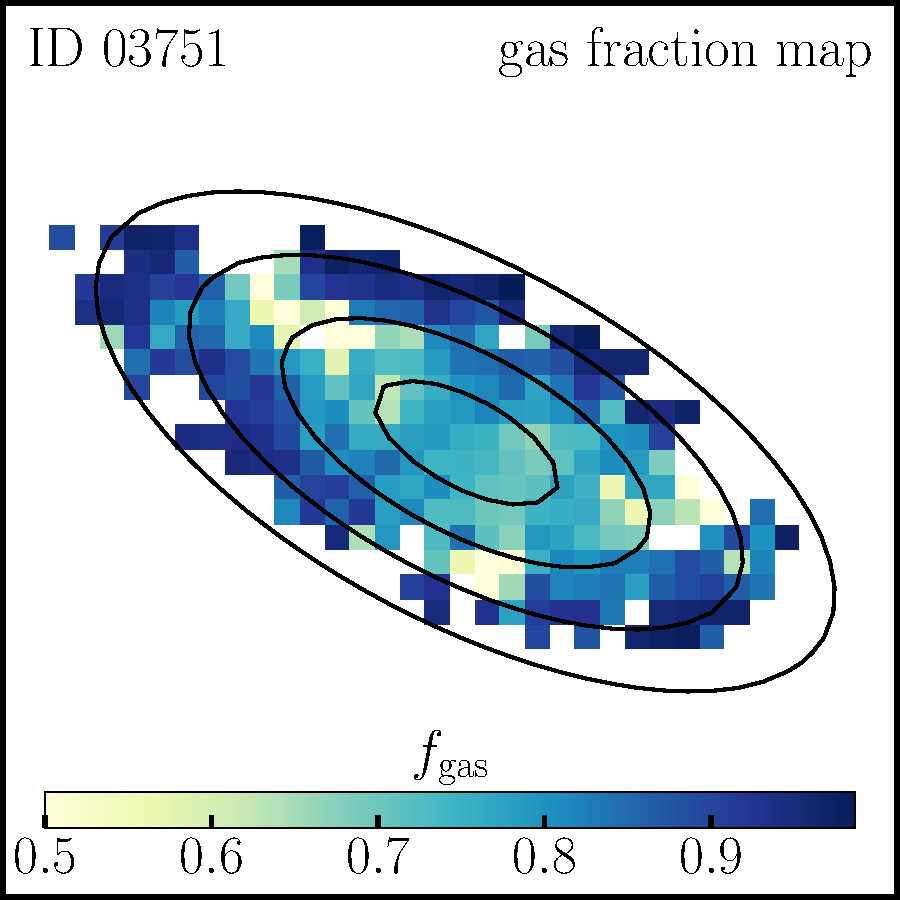
\includegraphics[width=.33\textwidth]{fig/physmap_fgas_ID03751.pdf}\\
    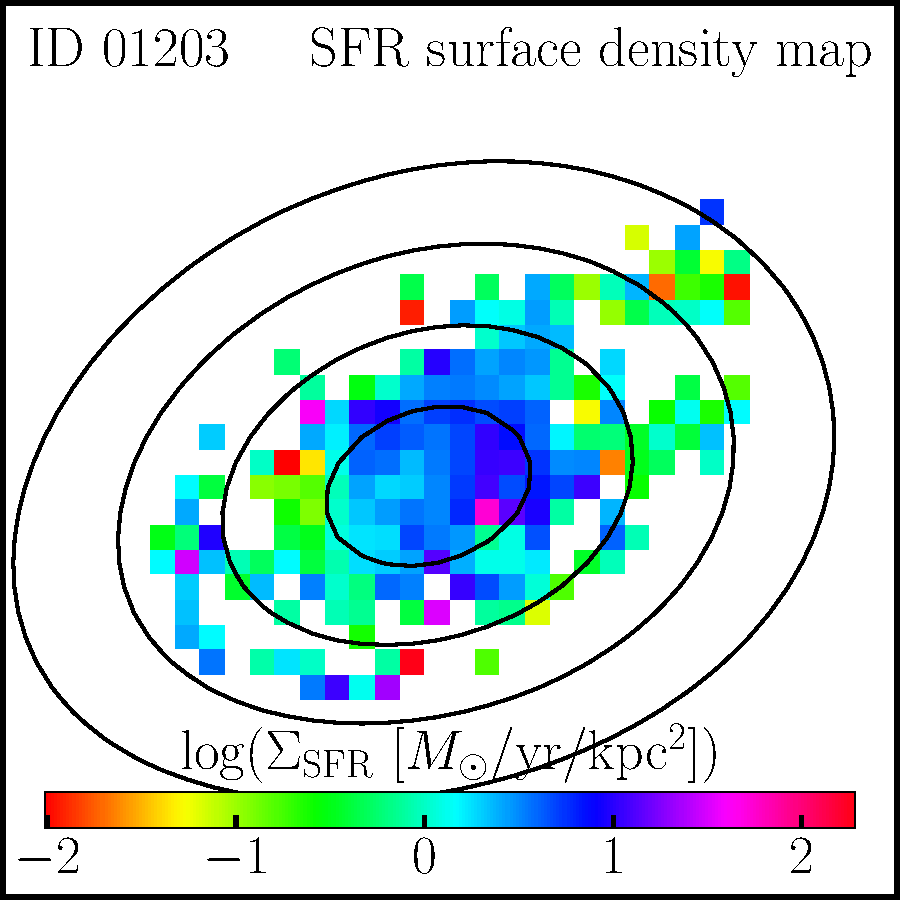
\includegraphics[width=.33\textwidth]{fig/physmap_lsfr_ID01203.pdf}
    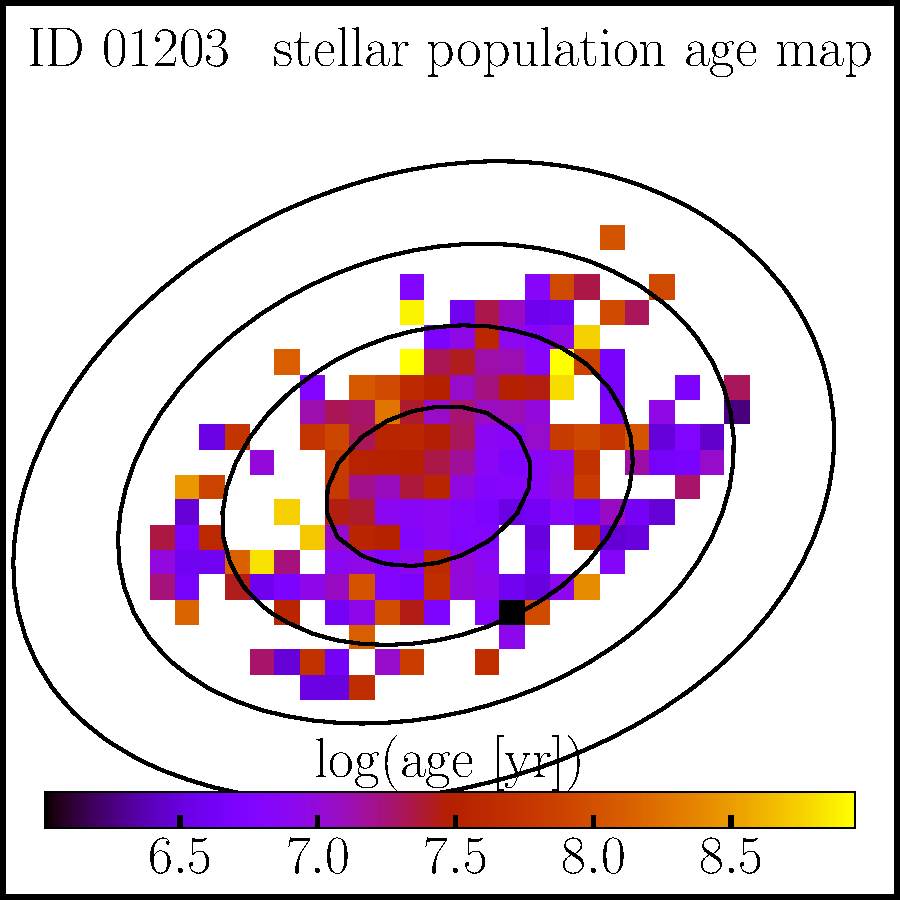
\includegraphics[width=.33\textwidth]{fig/physmap_lage_ID01203.pdf}
    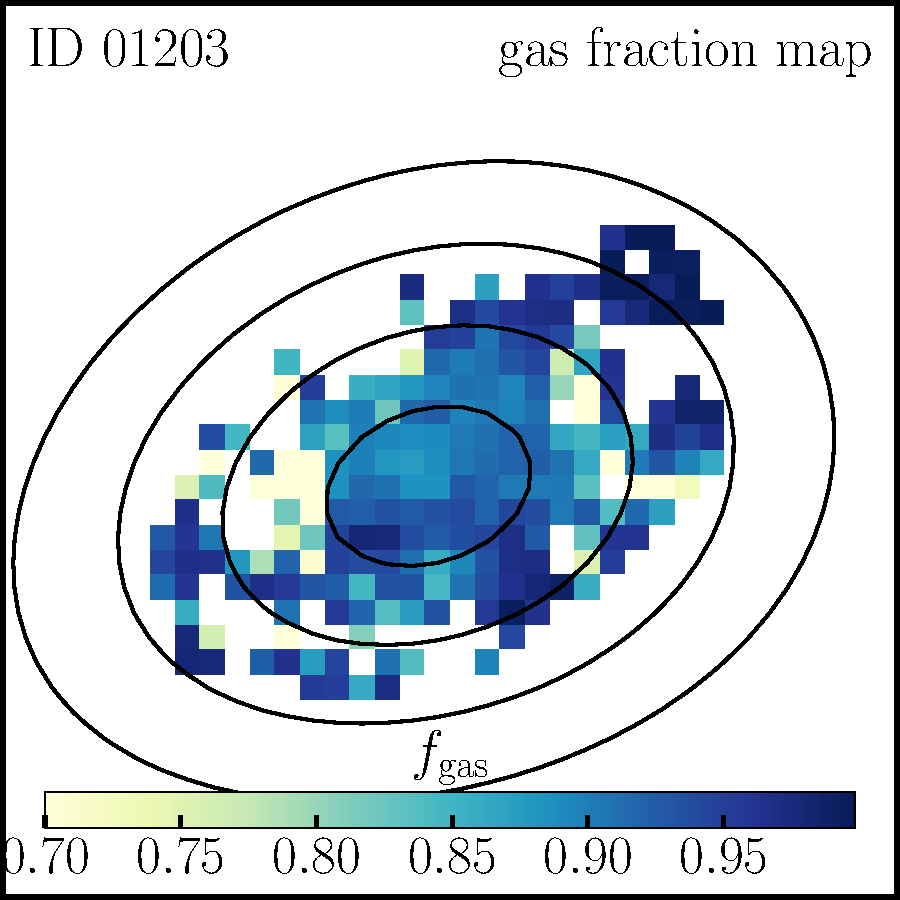
\includegraphics[width=.33\textwidth]{fig/physmap_fgas_ID01203.pdf}
    \caption[Maps of SFR surface density, average stellar population age, and gas fraction for our galaxies,
    derived from our spatially resolved analysis of stellar continuum and nebular emission.]
    {Maps of SFR surface density, average stellar population age, and gas fraction for our galaxies, derived from our
    spatially resolved analysis of stellar continuum and nebular emission.
    The spatial extent and orientation follows that in Figure~\ref{fig:combELmap}.
    We see that for both sources compared with their outskirts, their central regions have more active star formation, older 
    stellar population, and lower gas fraction.
    \label{fig:physmap}}
\end{figure}
%= = = = = = = = = = = = = = = = = = = = = = = = = = = = = = = = = = = = = = = =

As in \citet{Cresci:2010hr}, we compare our radially averaged \fgas and metallicity measurements against the predictions from
the simple chemical evolution model developed by \citet{Erb:2008di}.
To separate the effects of gas inflows and outflows, we compute two extreme sets of models, one being pure gas 
accretion (\ie with no outflows, $f_o=\Psi/\SFR=0$) and the other corresponding to the leaky box model (\ie with 
no inflows, $f_i=\Phi/\SFR=0$).
The results are shown in Figure~\ref{fig:Zerb_fgas}.
We note that for the pure gas accretion scenario, \fgas cannot decrease beyond a certain value, \ie,
$$
    \fgas^{\rm min} = 1-\frac{1-R}{f_i - f_o}
$$
where $f_o=0$ and $R$ is the instantaneous return fraction. This $\fgas^{\rm min}$, implicitly imposed by Eq.~(11) of 
\citet{Erb:2008di}, physically indicates that galaxies cannot exhaust their gas reservoir to below a certain amount without the 
help of outflows,
under the equilibrium condition with steady gas accretion (see Section~\ref{sect:regulator} when this equilibrium assumption is 
relaxed).
Therefore, the pure gas accretion scenario cannot explain the observed gas fractions in our source central regions (at $\lesssim$ 
2\kpc) where metallicities are also lower.
The leaky box model, on the other hand, provides a plausible explanation for our observation such that the outflow rate tends to 
increase towards galaxy center.
However, we stress that in reality both gas outflows and inflows are acting together to re-distribute 
metallicity. This test using simple chemical evolution models just clearly shows that using gas accretions 
\emph{alone} cannot explain our spatially resolved measurements.

%= = = = = = = = = = = = = = = = = = = = = = = = = = = = = = = = = = = = = = = =
%%% Figure:
\begin{figure}
    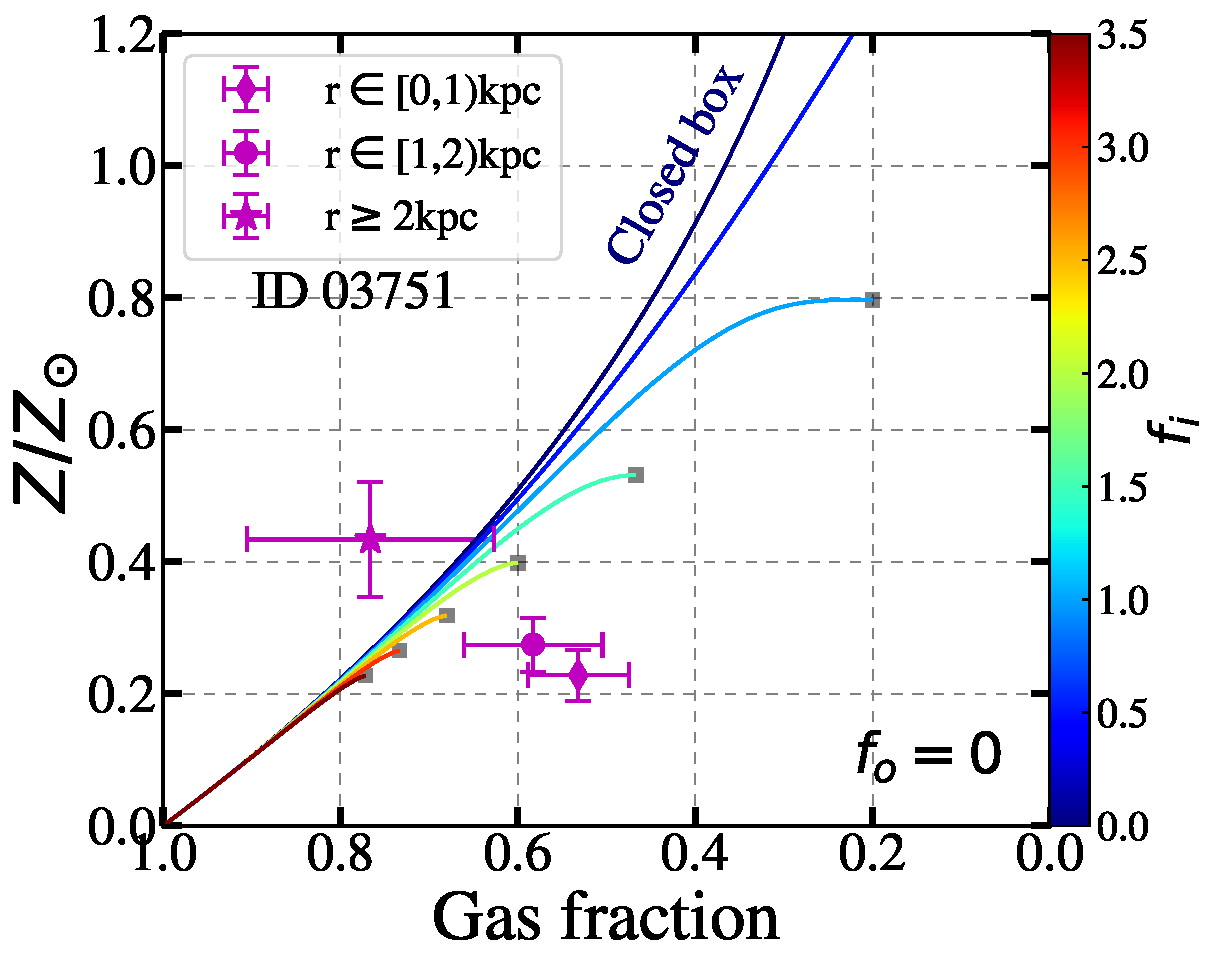
\includegraphics[width=.5\textwidth]{fig/Zerb_fgas_fixf_o.pdf}
    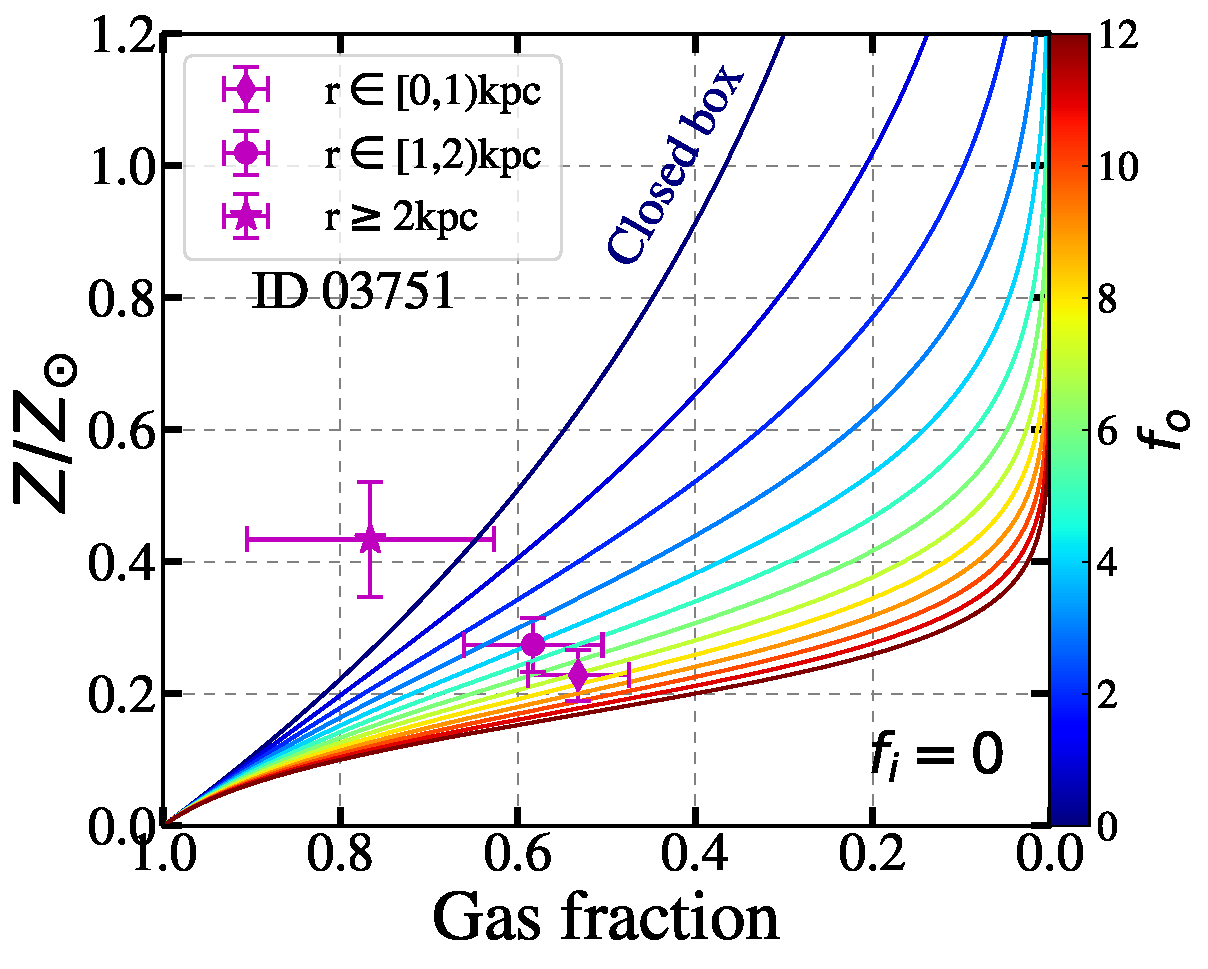
\includegraphics[width=.5\textwidth]{fig/Zerb_fgas_fixf_i.pdf}
    \caption[Gas fraction and metallicity estimated in different radial annuli.]
    {Gas fraction and metallicity estimated in different radial annuli for galaxy ID03751.
    The diamond, circle, and star symbols represent measurements derived at a galacto-centric radius of $r\in[0,1)$\kpc,
    $r\in[1,2)$\kpc, and $r\gtrsim2$\kpc, respectively.
    We also overlay the curves calculated from a simple chemical evolution model \cite{Erb:2008di} under extreme conditions, \ie,
    pure gas inflow ($f_o=0$; left) and pure gas outflow ($f_i=0$; right).
    Note that the trajectories of pure gas inflow cases cease at the grey squares for high infall rate ($f_i\gtrsim1$) conditions;
    any extensions from those grey squares toward low gas fraction (while fixing metallicity) are unphysical.
    This simple comparison shows that purely gas accretion does not suffice to explain the strong inverted gradients seen in our
    galaxies.
    \label{fig:Zerb_fgas}}
\end{figure}
%= = = = = = = = = = = = = = = = = = = = = = = = = = = = = = = = = = = = = = = =

\subsection{Spatially Resolved Gaseous Outflows}\label{sect:regulator}

%= = = = = = = = = = = = = = = = = = = = = = = = = = = = = = = = = = = = = = = =
%%% Figure:
\begin{figure}
    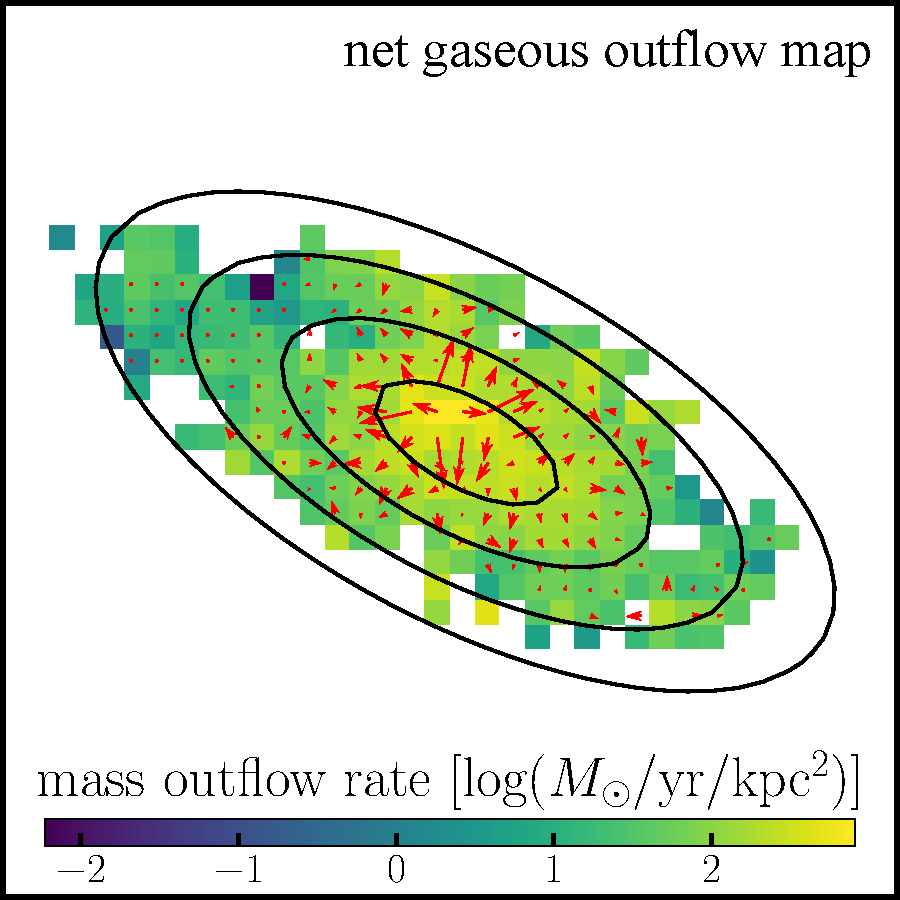
\includegraphics[width=.5\textwidth]{fig/outmass_ID03751.pdf}
    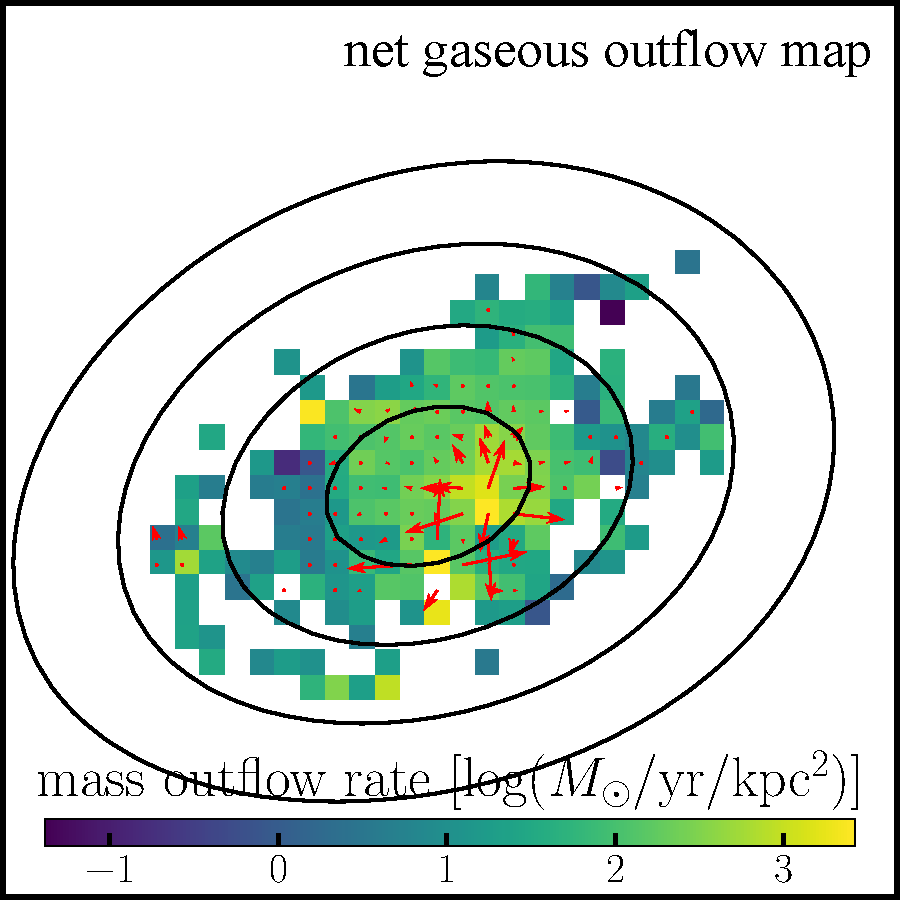
\includegraphics[width=.5\textwidth]{fig/outmass_ID01203.pdf}
    \caption[First ever maps of gaseous outflow rates at $z$$\sim$2.]
    {Maps of gaseous outflow rates derived from our analysis combining gas regulator models and empirical star-formation laws.
    The spatial extent and orientation follows that in Figure~\ref{fig:combELmap}.
    Red arrows show the net direction and magnitude of the gaseous outflows driven by galactic winds.
    We argue that outflows play a key role in effectively transporting stellar nucleosynthesis yields from the inner regions of 
    these two galaxies to their outskirts.
    \label{fig:outmass}}
\end{figure}
%= = = = = = = = = = = = = = = = = = = = = = = = = = = = = = = = = = = = = = = =

The application of simple chemical evolution in Section~\ref{sect:physprop} is enlightening but depends on 
strong assumption, such as that the azimuthal variations are negligible and galaxies live in equilibrium.
In reality, these conditions might not be valid, \eg, due to rapid gas flows.
To gain a more precise understanding of the physics of galactic winds and the role of gaseous outflows in 
shaping the observed spatial distribution of metallicity, independent of those assumptions, we can turn to a
more advanced framework for galaxy chemical evolution: the gas regulator model 
\citep{Lilly:2013ko,Peng:2014hn}.
This model provides an informative and coherent view of the full baryon cycle, involving the accretion of underlying DM halos, as 
well as the instantaneous regulation of star formation by a time-variable gas reservoir.
A key feature of this model is that it does not assume that galaxies live in an equilibrium state, where the total amount of gas 
mass remains constant. The non-equilibrium flexibility is especially important for applying this model to spatially resolved 
regions within a galaxy, where gas may be transported radially from one region to another. Chemical evolution within the gas 
regulator model is described by the equations
\begin{align}
    Z_{\rm gas} & = \left[Z_0 +
    y\taueq\epsilon\(1-\exp(-\frac{t}{\taueq})\)\right]\left[1 -
    \exp(\frac{-t/\taueq}{1-\exp(-t/\taueq)})\right],      \\
    \tau_{\rm eq} & = \frac{1}{\epsilon\(1-R+\lambda\)}.    \non
\end{align}
Here we adopt the convention of symbols itemized in Table~1 of \citet{Peng:2014hn}:
\Zgas is the mass fraction of metals in the gas reservoir (determined from the observed \oh as in \citet{Peeples:2011ew}), $t$ is 
the average stellar population age, $\taueq$ is the time scale on which the baryon cycle reaches equilibrium, $\epsilon$ is the 
\sf efficiency (defined as $\epsilon\equiv\SFR/\Mgas=\Sigma_\SFR/\Sgas$), and $\lambda$ is the mass loading factor (defined in 
terms of the mass outflow rate $\Psi$, such that $\lambda=\Psi/\SFR$\footnote{Note that $\lambda$ and $f_o$ in 
Section~\ref{sect:physprop} represent the same quantity but here we are solving for $\lambda$ in a spatially resolved fashion.}).
We adopt a stellar nucleosynthesis yield $y=0.003$ \citep{Dalcanton:2007kc} with $R=0.4$ estimated from BC03 
\citep{Bruzual:2003ck} stellar population models. Finally, we assume that gas inflows are pristine ($Z_0=0$).

For each spatial region where we have estimated the metallicity, \SFR, gas surface density, and age (Figures~\ref{fig:oh12grad}, 
\ref{fig:physmap}), we solve the above equations for the mass loading factor $\lambda$ and subsequently calculate the mass outflow 
rate $\Psi$.
The 2D distribution of $\Psi$ is displayed in Figure~\ref{fig:outmass}.
Taking the gradient field of this gaseous outflow map, we obtain the net direction of the outflowing mass flux on 
sub-galactic scales, projected along the line of sight, denoted by the red arrows in Figure~\ref{fig:outmass}.
The results demonstrate that strong galactic winds transport mass from the center to the outskirts, with the net 
radial transport of heavy elements causing the inverted gradients observed in our targets.

%= = = = = = = = = = = = = = = = = = = = = = = = = = = = = = = = = = = = = = = =
%%% Figure:
\begin{figure}
    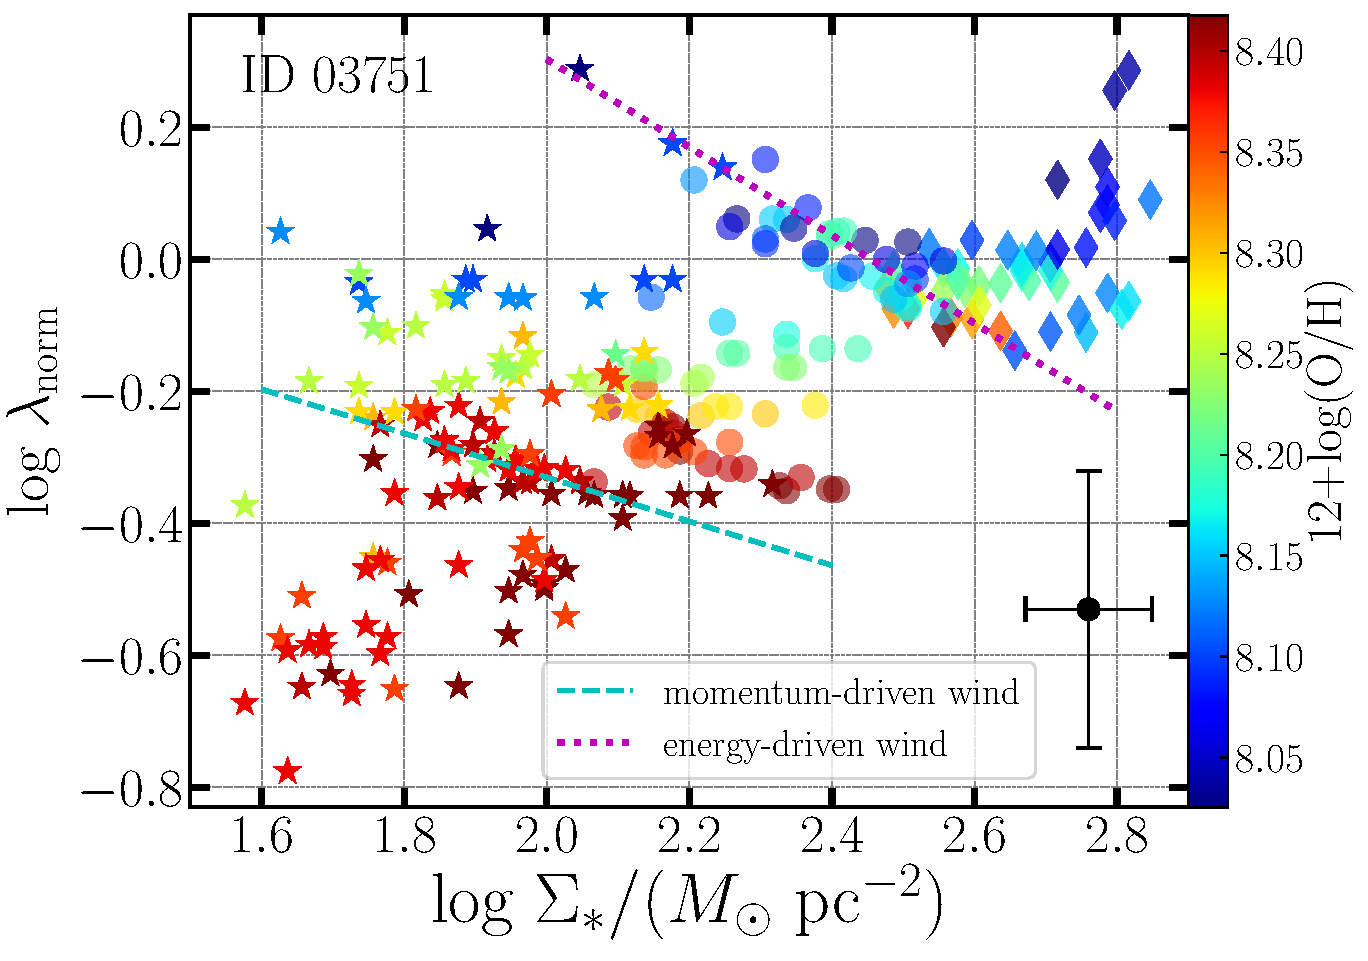
\includegraphics[width=.5\textwidth]{fig/lamSDstar_ID03751.pdf}
    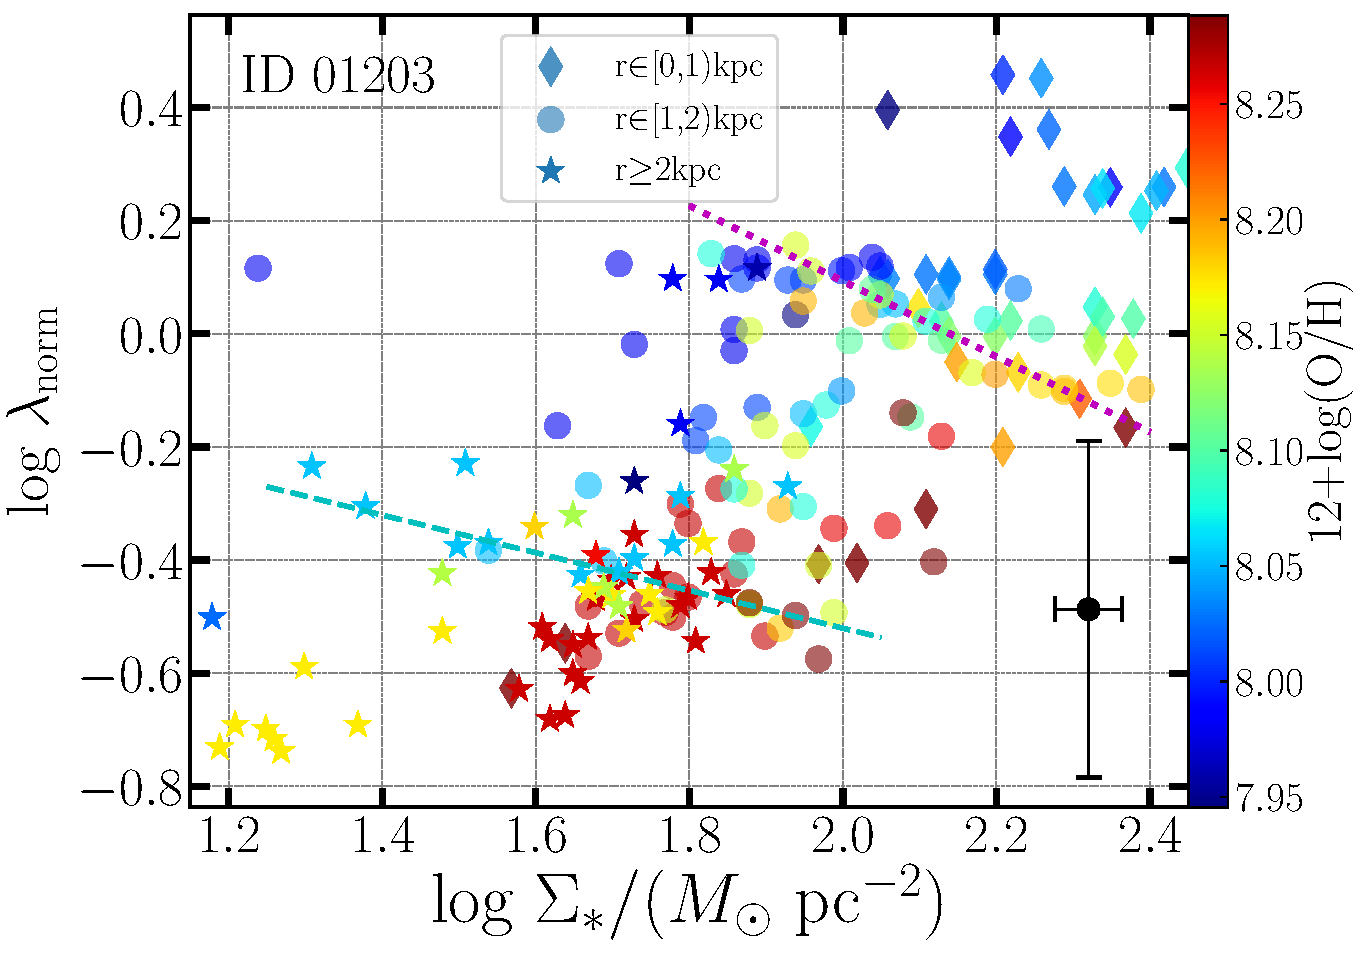
\includegraphics[width=.5\textwidth]{fig/lamSDstar_ID01203.pdf}
    \caption[Correlation between spatially resolved mass loading factor and stellar surface density.]
    {Correlation between spatially resolved mass loading factor $\lambda$ (normalized to the value at radius 1
    kpc; see Table~\ref{tab:srcprop}) and stellar surface density $\Sigma_\ast$, color-coded by metallicity.
    As in Figure~\ref{fig:physmap}, the diamond, circle, and star symbols represent measurements derived at a 
    galacto-centric radius
    of $r\in[0,1)$\kpc, $r\in[1,2)$\kpc, and $r\gtrsim2$\kpc, respectively.
    We overlay as an illustration two scaling relations that are commonly assumed to describe integrated measurements:
    $\lambda\propto\Sigma_\ast^{-2/3}$ for an energy-driven wind model marked by magenta dotted lines, and
    $\lambda\propto\Sigma_\ast^{-1/3}$ for a momentum-driven wind model by cyan dashed lines.
    Evidently, a single scaling relation is not sufficient to describe the spatially resolved data, demonstrating the need for a
    more sophisticated approach.
    The black point in the lower right corner in each panel displays the median uncertainties for these measurements.
    \label{fig:lamSDstar}}
\end{figure}
%= = = = = = = = = = = = = = = = = = = = = = = = = = = = = = = = = = = = = = = =

The distribution of mass loading factors $\lambda$ within each of our targets is also shown in 
Figure~\ref{fig:lamSDstar}, revealing higher $\lambda$ (and therefore a higher fraction of metals lost) in the central regions.
This preferential removal of metals from the center, and subsequent deposition at larger radii, gives rise to the strong 
positively sloped metallicity gradients evident in Figure~\ref{fig:oh12grad}.
The high values of $\lambda$ have important implications for the role of feedback in galaxy formation.
Most fundamentally, our results support feedback as a solution to the ``over-cooling'' problem in galaxy formation, by ejecting
gas and preventing overly condensed baryonic regions at high redshifts \citep{1978MNRAS.183..341W,Dekel:1986cv}.
Such strong outflows are also expected to suppress the formation of stellar bulges from low angular momentum gas 
\citep{Governato:2010ed,Brook:2012gj}.
This is consistent with low bulge fraction in these two galaxies measured from high resolution \hst imaging 
(Table~\ref{tab:srcprop}).

%A tantalizing feature in the $\lambda$ distribution is the co-existence of multiple wind modes {\em within} individual galaxies.
A key feature in the $\lambda$ distribution is that neither of the wind modes, driven by momentum or energy conservation, can 
explain the behavior of the mass dependence of $\lambda$ alone, {\em within} individual galaxies.
Outflows are typically parameterized by either a momentum-driven \citep{Oppenheimer:2006eq,Oppenheimer:2008bu} or an
energy-driven \citep{Springel:2003eg} wind mode, both of which are physically well motivated \citep{Murray:2005jt}.
The energy-driven wind scenario assumes that outflows are launched by the thermal pressure of supernova (SN) explosions and/or
winds from massive stars.
A portion of this thermal energy provides the outflow kinetic energy, \ie, $\Psi\times v^2_{\rm wind} \sim \SFR$, where the wind 
speed $v_{\rm wind}$ can mimic the escape velocity from DM halo, \ie, $v_{\rm esc}\sim M_{\rm h}^{1/3}$ given by the virial 
theorem.
This results in the scaling relation of $\lambda\propto\Mstar^{-2/3}$, assuming the linear correlation between the mass 
constituents of stellar and dark components.
The energy-driven wind model is found successful in explaining the low abundance of satellite galaxies in the Milky Way 
\citep{Okamoto:2010ba}.
The momentum-driven wind model instead relies on the momentum injection deposited by radiation pressure from SN explosions and/or 
massive stars, leading to $\Psi\times v_{\rm wind} \sim \SFR$ and $\lambda\propto\Mstar^{-1/3}$.
In this scenario, $v_{\rm wind}$ is proportional to \Mstar and \SFR, broadly consistent with some observational
results \citep{Martin:2005kx}.
The transition from energy- to momentum-driven winds is typically thought to be a galaxy-wide phenomenon,
resulting in the steepening of the mass-metallicity relation below \Mstar~$\simeq10^{9.3}$\Msun at $z\simeq2$ 
\citep{Henry:2013gx}.
However, our analysis indicates that a single mode is not sufficient to describe spatially resolved data \emph{within} one galaxy 
and it is highly likely that the transition from energy- to momentum-driven winds occurs on sub-galactic scales, governed by local 
gas and star formation properties in addition to the global gravitational potential.
%Specifically the data in the central region appear to cluster around the more powerful energy-driven scaling, while the outskirts 
%are roughly in the region covered by the scaling for a momentum-driven wind.


\section{Summary and Discussion}\label{sect:conclu}

We present the first robust confirmation of the existence of strongly inverted metallicity radial gradient (\ie $\gtrsim$0.1 
dex/kpc) in star-forming dwarf galaxies ($\Mstar\lesssim10^9\Msun$) at the peak of star formation and chemical enrichment 
($z\sim2$).
Our synergy of the diffraction-limited imaging spectroscopy from \hst NIR grisms and lensing magnification permits exquisite 
spatial sampling, \ie, at the scale of 50-100 pc, to securely resolve our $z\sim2$ galaxies with $\gtrsim$300 resolution elements 
(Figures~\ref{fig:combELmap} and \ref{fig:oh12grad}) to deliver precise radial gradient measurements.
To understand the physical origin of these strongly inverted gradients, we obtain high resolution 2D maps of star formation rate, 
characteristic stellar age (or equivalently star formation timescale), and gas fraction, from \hst observations of source stellar 
continuum and nebular emission.
These 2D maps show that the galactic disks of our sources are rapidly assembling stellar mass through in-situ star formation, in 
the early phase of inside-out growth (Figure~\ref{fig:physmap}).
By comparing our observations with simple chemical evolution models, we find that gas accretion alone cannot explain these 
strongly inverted gradients in our galaxies (Figures~\ref{fig:Zerb_fgas}).

Using a more advanced gas regulator model, we are able to calculate the spatial distribution of mass loss rates from outflows, 
treating each spaxel as an independent star-forming region, and thus map the macroscopic patterns of net gaseous outflows 
(Figure~\ref{fig:outmass}).
It turns out that the mass loss rates are highest in the central regions of both galaxies, coincident with
the peak star formation surface densities.
A natural explanation is thus that active star formation in galaxy centers gives rise to powerful winds that transport gas and
metals away from the center toward larger radii, forming ``galactic fountains'' \citep{Martin:2002ee}.

Furthermore, our spatially resolved analysis of metals, \SFR, and stellar populations shows that a single type of wind mechanism 
(either energy or momentum driven) cannot explain the entire galaxy (Figure~\ref{fig:lamSDstar}).
A primary physical parameter that has been proposed to set the transition between the two wind dynamics is the gravitational 
potential, often parameterized by velocity dispersion ($\sigma$). There exists a critical scale \scrit 
\citep{Murray:2005jt} such that for galaxies with $\sigma<\scrit$, energy injection by SNe sets a limiting 
\SFR above which interstellar gas is ejected in galactic winds. For galaxies with $\sigma>\scrit$, momentum 
deposition limits the maximum \SFR above which the ISM is likewise ejected.
The presence of both energy- and momentum-driven wind scalings in one galaxy suggests that feedback-triggered winds are connected
to physical properties on sub-galactic scales, \eg, \emph{local} velocity dispersion ($\sigma_{\rm local}$), 
which is sensitive to the optical depth of gas flows, the coupling efficiency between gas clouds and dust 
parcels, \etc.
On sub-galactic scales, there exists a strong correlation among velocity dispersion (not necessarily 
$\sigma_{\rm local}$), surface density and size of molecular clouds \cite[see][and references 
therein]{BallesterosParedes:2011gk}.
It appears that in our galaxies, the wind-launching mechanism transitions from energy- to momentum-driven as 
galacto-centric radius increases.
This gives rise to a hypothesis that $\sigma_{\rm local}$ in our galaxies should increase from inner to outer 
regions.
%straddling a critical value similarly defined as $\scrit$.
Our current kinematic data on source ID01203 have high spatial resolution (at $0\farcs05$ plate scale) yet narrow FoV so that it 
is infeasible to map sub-kpc scale velocity dispersion accurately to outer regions at $r\gtrsim2$ \kpc, where momentum-driven wind 
seems to take over.
To test this hypothesis conclusively, more spatially resolved data taken under sufficient spatial sampling will be required to 
robustly derive a full 2D map of velocity dispersion out to the periphery of the galactic disk, using instruments 
with relatively large FoV, \eg, the \jwst NIRSpec IFU \citep{Kalirai:2018gs}.

Physically, the momentum-driven wind scaling applies to ``cool'' ($T \sim 10^4$ K) ambient interstellar gas entrained in outflows,
whereas the energy-driven wind is appropriate when entrained gas is shock heated to temperatures where cooling is inefficient ($T
\sim 10^6$ K). A plausible scenario for our galaxies is that feedback from an intense burst of star formation in the central
regions heats the ejected gas to a highly ionized phase, while gas entrained in outflows from the outer regions remains cool. If
this interpretation is correct, then we expect a distinct signature in the absorption properties of outflowing gas. Outflows from
the central regions should be dominated by highly ionized species (e.g. \ionp{O}{vi}, \ionp{C}{iv}, \ionp{Si}{iv}) whereas
outflows from the outer regions should have relatively more of the low ions characteristic of $T \sim 10^4$ K gas (e.g.
\ionp{Fe}{ii}, \ionp{Mg}{ii}, \ionp{Si}{ii}). Both high and low ion species are commonly observed in outflows from star forming
galaxies at $z\simeq2$ \citep{Berg:2018gd,Du:2018tr}, although their spatial distributions are not yet well known 
\citep[but see][]{James:2018km}.
Our hypothesis suggests a more central concentration of the high ions \emph{in the specific cases} where a 
combination of both outflow scalings results in inverted metallicity gradients.
This prediction can be directly tested with spatially resolved spectroscopy of rest-frame
ultraviolet absorption lines using instruments such as \keck/KCWI or VLT/MUSE.


          % Chapter 2
%\input {chapter3}
%\input {chapter4}
%\input {chapter5}
%\input {chapter6}
%\input {chapter7}
%\input {chapter8}


\bibliographystyle{modapj}
\bibliography{bibtexlib}

\end{document}

